\documentclass{article}

\usepackage[T1]{fontenc}    %Schriftart des Dokumentes
\usepackage[ngerman]{babel} %Dokumentensprache, hier Deutsch
\usepackage{amsmath, amssymb, stmaryrd} %mathematische Schriftzeichen
\usepackage{graphicx} %Einfügen von Grafiken
\usepackage{wrapfig}
\usepackage{bm}
\usepackage{subfig}
\usepackage{newclude}
\usepackage{pdfpages}

\setlength{\parindent}{0pt} %Einrückung von Absätzen auf null gesetzt
\setlength{\parskip}{10pt} %Abstand zischen Absätzen auf 10pt gesetzt

\title{Versuch 222: Heißluftmotor}
\author{Matthias Kuntz}
\date{04.03.2024}

\renewcommand*\contentsname{Zusammenfassung}

\begin{document}

\maketitle

\tableofcontents

\newpage

%-------------------------EINLEITUNG-------------------------
\section{Einleitung}

Erstmals 1816 vom schottischen Pfarrer Robert Stirling vorgestellt war der Heißluftmotor eine Erfindung, die die damals populär gewordenen gefährlichen Hochdruckdampfmaschinen ablösen sollte. Mit dem Ziel einen effizienten und sichereren Motor zu erschaffen, entwickelte Stirling das Konzept eines Motors, der von außen Wärme erhält und diese in mechanische Arbeit umwandelt. Jedoch hatte der Motor zunächst nicht den gewünschten Erfolg. Gegen die steigende Sicherheit und damit Popularität der Dampfmaschinen  kam er nicht an, bis dann schlussendlich der Verbrennermotor das Ende für den Sirlingmotor verheißen sollte. Aber die Idee des umweltfreundlichen und vielseitig einsetzbaren Motors verschwand nicht. Gerade in den letzten Jahren gewann er wieder an Popularität, da er mit seiner umweltschonenderen Betriebsweise und seinem hohen potientiellen Wirkungsgrad eines Tages eine realistische Alternative zu klassischen Verbrennermotoren werden könnte. Auch die Möglichkeit mit einem Stirlingmotor in umgekehter Betriebsweise, ergo durch die Zufuhr von Arbeit, Wärme oder Kälte zu generieren, macht ihn zur interessanten Energiequelle. In diesem Versuch soll es also um die grundlegenden Funktionsweisen sowie den einfachen Betrieb eines Heißluftmotors gehen und es sollen dessen Effizienz und Leistung untersucht werden.

\subsection{Physikalische Grundlagen}

\subsubsection{Wirkungsweise eines Heißluftmotors}

Der einfachste Ansatz, um eine Gespür für die Funktionsweisen eines Stirlingmotors zu bekommen, ist, indem man sich den Aufbau eines sogenannten $\gamma$-Typ Heißluftmotors anschaut. Dieser bestitzt nämlich, nicht so wie der in diesem Versuch später verwendete Stirlingmotor, zwei verschiedene Zylinder für die beiden verschiedenen Prozesse, wodurch diese anschaulicher werden. Eine kleine schematische Zeichnung des Aufbaus ist in Abbildung \ref{fig:schema_gamma} zu sehen. 

\begin{figure}[!h]
    \centering
    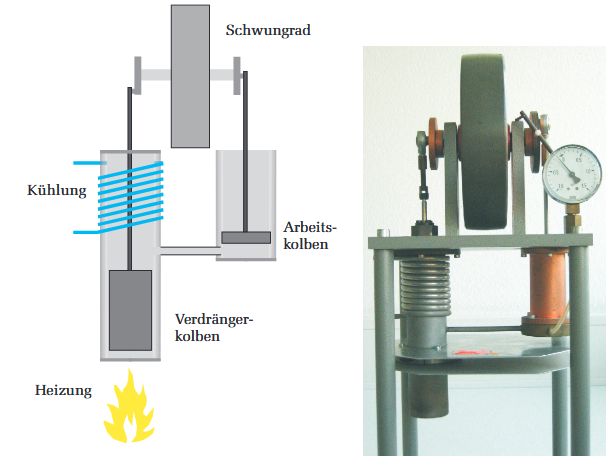
\includegraphics[width=0.8\textwidth]{graphics/einleitung/gamma.png}
    \caption{Aufbau eines $\gamma$-Typ Heißluftmotors [Quelle: PAP2.1 Skript, S.37, 11.03.2024]}
    \label{fig:schema_gamma}
\end{figure}

Im Grunde funktioniert der Aufbau dabei wiefolgt: In den beiden Zylindern ist jeweils ein Kolben, einmal ein Verdrängerkolben im linken und ein Arbeitskolben im rechten. Die beiden sind über ein Schwungrad verbunden. Der Verdrängerkolben im linken Zylinder hat nun die Aufgabe, das Gas links abwechselnd von oben nach unten im Zylinder zu verschieben. Dabei wird das Gas im oberen Bereich abgekühlt und im unteren aufgeheizt. Je nachdem wo sich das Gas befindet steigt oder sinkt somit sowohl die Temperatur, als auch damit verbunden der Druck. Wichtig ist, dass der Verdrängerkolben das Gas niemals komprimiert, sondern einfach nur verschiebt. Die Kompression beziehungsweise Expansion ist nämlich die Aufgabe des Arbeitskolben im anderen Zylinder. Dieser ist so am Schwungrad angeordnet, dass immer dann Kompression stattfindet, wenn der Verdrängerkolben das Gas in den kalten Bereich geschoben hat. Da die Zylinder über ein Rohr verbunden sind, komprimiert der Arbeitskolben somit das kalte Gas bei geringem Druck. Verschiebt der Verdrängerkolben nun das Gas in den warmen Bereich, so steigt der Druck und schiebt den Arbeitskolben nach oben, wodurch nach außen mechanische Arbeit geleistet wird. Danach kühlt das Gas wieder ab und ein Teil der Arbeit wird genutzt, um das Gas wieder zu komprimieren. So beginnt der Kreisprozess erneut.   

Der Unterschied zu dem in diesem Versuch verwendeten Stirlingmotor ist nun wie bereits erwähnt, dass hier beide Kolben in einem einzigen Zylinder stecken. Laut spezieller Klassifizierung ist dies dann ein $\beta$-Typ Stirlingmotor, zu sehen in Abbildung \ref{fig:schema_beta}. Grundlegend funktioniert dieser Motor aber auf gleiche weise, der Unterschied ist nur, dass der Gasaustausch nun nicht mehr über ein Rohr, sondern direkt im selben Zylinder erfolgt. Der Vorteil davon ist, dass sich somit das Gesamtvolumen verringert und so der Wirkungsgrad steigt. 

\begin{figure}[!h]
    \centering
    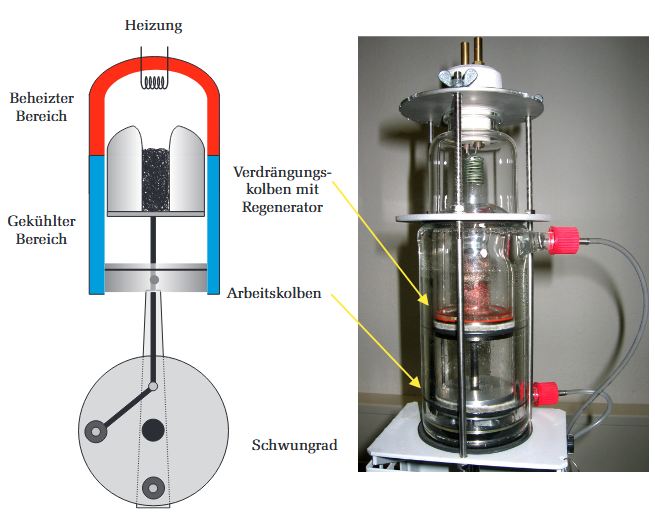
\includegraphics[width=0.8\textwidth]{graphics/einleitung/beta.png}
    \caption{Aufbau eines $\beta$-Typ Heißluftmotors [Quelle: PAP2.1 Skript, S.37, 11.03.2024]}
    \label{fig:schema_beta}
\end{figure}

Ein weiterer Aspekt, der bei dem verwendeten Stirlingmotor für einen besseren Wirkungsgrad sorgt, ist der ebenfalls in Abbildung \ref{fig:schema_beta} zu sehende Regenerator. Besitzt der Verdrängerkolben eine mit Kupferwolle gefüllte Öffnung in axialer Richtung, so strömt bei Verschiebung des Gases zwischen den warmen und kalten Bereichen das Gas durch die Kupferwolle. Bewegt sich der Verdränger beispielsweise nach oben, so strömt die warme Luft durch den Regenerator und gibt Wärme an die Kupferwolle ab. Dadurch kühlt das Gas nicht nur schneller ab, sondern kann auf genau diese Wärme beim Rückweg, wenn sich der Kolben wieder nach oben bewegt, zurückgreifen und sich somit auch wieder schneller erwärmen. Insgesamt erziehlt man also, dass zum Einen mehr Wärme im System erhalten bleibt und nicht an das Kühlsystem verloren geht und zum Anderen wird ein schnellerer Temperaturwechsel des Arbeitsgases ermöglicht, was beides den Wirkungsgrad des Stirlingmotors ehöht, im Idealfall sogar bis zum maximal möglichen Wirkungsgrad einer periodisch arbeitenden Wärmekraftmaschine. 

\newpage
\subsubsection{Der ideale Stirling-Prozess}

Wir möchten nun qualitativ und quantitativ beschreiben, was genau in einem Heißluftmotor während einer Umdrehung passiert. Dazu wiederholen wir zunächst ein paar Grundlagen, die für die gleich folgenden Berechnungen relevant werden.

Wir erinnern uns zunächst an die Zustandsgleichung des Idealen Gases, welche die Größen Volumen $V$, Druck $p$, Temperatur $T$, und Gasmenge $\nu$ [mol] über die ideale Gaskonstante $R$ verbindet:

\begin{equation}
    pV = \nu R T.
    \label{eq:idealesGasgesetz}
\end{equation}

Auch wichtig wird der Erste Hauptsatz der Thermodynamik: Wird einen System die Wärmemenge $dQ$ zugeführt, so kommt es zu einer Änderung der inneren Energie $dU$ sowie zu einer verrichteten Volumenarbeit $p \ dV$:

\begin{equation}
    dQ = dU + p \ dV.
    \label{eq:1.HS_Thermodynamik}
\end{equation}

Im Falle eines idealen Gases setzt sich die innere Energie allein aus der Bewegungsenergie der Gasmoleküle zusammen. Somit führt eine Änderung der inneren Energie zu einer proportionalen Änderung der Temperatur, gegeben über die molare Wärmekapazität $C_V$:

\begin{equation}
    dQ = \nu C_V \ dT + p \ dV.
\end{equation}

Zuletzt möchten wir noch an die grundlegenden Begriffe der thermodynamischen Prozesse erinnern:

\begin{itemize}
    \item[-] isotherm: Temperatur konstant ($pV =$ konst.)
    \item[-] isochor: Volumen konstant ($V =$ konst.)
    \item[-] isobar: Druck konstant ($p =$ konst.)
    \item[-] adiabatisch: Kein Wärmeaustausch mit der Umgebung ($pV^\kappa =$ konst.)
\end{itemize}

Mit diesen Grundlagen können wir nun den Stirling-Prozess verstehen. Dazu betrachten wir die vier nacheinander ablaufenden Prozesse dargestellt in Abbildung \textbf{!!!!}. Links sieht man das zugehörige pV-Diagramm und rechts die jeweilige Stellung der Kolben. Beim idealen Stirling-Prozess werden nacheinander die folgenden Zustandsänderungen durchlaufen.

\begin{figure}[!h]
    \centering
    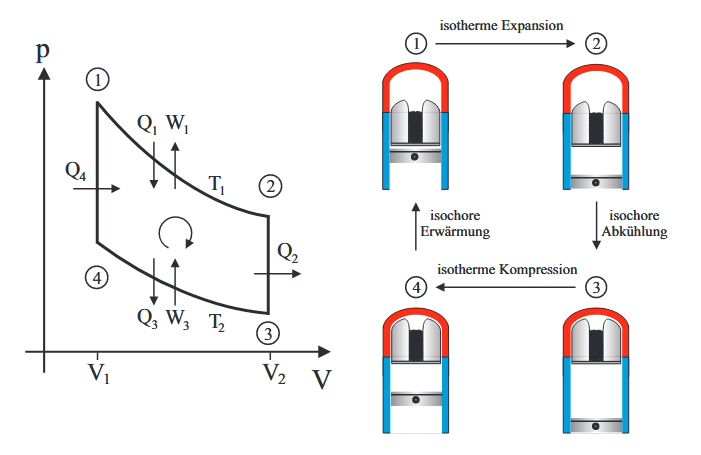
\includegraphics[width=0.8\textwidth]{graphics/einleitung/stirlingprozess.png}
    \caption{Idealer Stirlingprozess; links: pV-Diagramm, rechts: Stellung der Kolben [Quelle: PAP2.1 Skript, S.38, 11.03.2024]}
    \label{fig:schema_beta}
\end{figure}

\begin{description}
   \item[1 $\xrightarrow{}$ 2: Istotherme Expansion] In Position 1 befindet sich der Verdrängerkolben ganz unten, ergo im unteren Totpunkt. Im Zylinder herrscht die Temperatur $T_1$ und das Gas nimmt im oberen Teil die dem Heizsystem entzogenen Wärme $Q_1$ auf, welche aufgrund der konstanten Temperatur (isotherm) komplett in mechanische Volumenarbeit umgewandelt wird, die den Arbeitskolben nach unten drückt. Das Gas leistet also die Arbeit $W_1$. Mathematisch lässt sich das ganze folgendermaßen Beschreiben: \\
   Das Gas wandelt die Wärme $Q_1$ in Volumenarbeit $p \phantom{.} dV$ um. Mit dem idealen Gasgesetz aus Gleichung \ref{eq:idealesGasgesetz} erhalten wir somit:

   \begin{equation}
       dQ_1 = p \phantom{.} dV = \nu R T_1 \frac{dV}{V}.
   \end{equation}

   Integrieren wir diesen Ausdruck von $V_1$ bis $V_2$, ergo einmal über die Gesamte Volumenänderung während des Prozesses, so erhalten wir die gesamte ins System eingeführte Wärmemenge $Q_1$:

   \begin{equation}
       Q_1 = \nu R T_1 \int_{V_1}^{V_2} \frac{dV}{V} = \nu R T_1 \ \ln{\left( \frac{V_2}{V_1} \right)}.
   \end{equation}

   Und da diese Wärmemenge komplett in die geleistete Volumenarbeit $W_1$ umgewandelt wird, erhalten wir für diese ebenso

   \begin{equation}
       W_1 = \nu R T_1 \ \ln{\left( \frac{V_2}{V_1} \right)}.
   \end{equation}

   \phantom{.}
   \item[2 $\xrightarrow{}$ 3: Isochore Abkühlung] Nachdem der Arbeitskolben nach ganz unten geschoben wurde bewegt sich der Verdrängerkolben nach oben und verschiebt somit das Gas aus dem geheizten zu dem gekühlten Bereich. Dabei kühlt sich das Gas auf die Temperatur $T_2$ ab und gibt somit die Wärmeemenge $Q_2$ an das Kühlsystem ab. Da sich der Arbeitskolben hier nicht bewegt ändert sich auch das Volumen nicht und es wird keine Volumenarbeit verrichtet ($dV = 0$). Somit gilt für die Innere Energie:

   \begin{equation}
       dQ_2 = - \nu C_V \ dT.
   \end{equation}

   Integriert man über die Temperaturänderung so erhält man die abgegebene Wärme $Q_2$:

   \begin{equation}
       Q_2 = - \nu C_V \int_{T_1}^{T_2} dT = - \nu C_V (T_2 - T_1).
   \end{equation}

   Da hier keine Volumenänderung stattfand ist die mechanische Arbeit bei diesem Motortakt $W_2$ entsprechend 

   \begin{equation}
       W_2 = 0.
   \end{equation}

   \phantom{.}

   \item[3 $\xrightarrow{}$ 4: Isotherme Kompression] Nun bewegt sich wieder der Abeitskolben. Er drückt die kalte Luft nach oben zusammen und muss dafür die Arbeit $W_3$ verrichten. Die dabei freiwerdende Wärmemenge $Q_3$ wird an das Kühlsystem abgeben. Mathematisch berechnet man die beiden Werte analog zum ersten Prozess, wobei nun natürlich die Temperatur $T_2$ im Kolben herrscht und das Gas umgekehrt von $V_2$ zu $V_1$ komprimiert wird. Man erhält somit:

   \begin{equation}
       Q_3 = W_3 = - \nu R T_2 \ \ln{\left( \frac{V_2}{V_1} \right)}.
   \end{equation}

   \phantom{.}
   \item[4 $\xrightarrow{}$ 1: Isochore Erwärmung] Im letzten Schritt bewegt sich der Verdrängerkolben wieder nach unten und schiebt das Gas nach oben in den geheizten Bereich. Dabei wird die Wärmemenge $Q_4$ aufgenommen um die Temperatur wieder auf den Anfangswert $T_1$ zu eröhen. Analog zum zweiten Prozess erhalten wir somit:

   \begin{equation}
       \begin{split}
           Q_4 &= \nu C_V (T_1 - T_2), \\
           W_4 &= 0.
       \end{split}
   \end{equation}

   Danach beginnt der Kreisprozess von vorne.
\end{description}

Die gesamte geleistete Nutzarbeit $W_N$ eines Kreislaufs ergibt sich nun aus dem Kurvenintegral über alle Prozesse. Da aber nur bei den isothermischen Prozessen Arbeit verrichtet wird, ergibt sie sich einfach aus der Summe der Beiden:

\begin{equation}
    \begin{split}
        W_N &= \oint p \ dV = W_1 + W_3 = \nu R (T_1 - T_2) \ln{\left( \frac{V_2}{V_1} \right)}
    \end{split}
    \label{eq:StirlingNutzarbeit}
\end{equation}

Mithilfe der Nutzarbeit kann nun der ideale thermische Wirkungsgrad $\eta_{th}$ aus dem Verhältnis zur aufgenommenen Wärmemenge $Q_+$ definiert werden:

\begin{equation}
    \eta_{th} = \frac{W_N}{Q_+}.
\end{equation}

Im Fall ohne Regenerator ergibt sich $Q_+$ einfach aus der Summe der im ersten und letzten Schritt aufgenommenen Wärmen $Q_1$ und $Q_4$. Somit erhalten wir nach einigen Umformungen und mit Gleichung \ref{eq:StirlingNutzarbeit}:

\begin{equation}
    \begin{split}
        Q_+ &= Q_1 + Q_4 = \nu R T_1 \ \ln{\left( \frac{V_2}{V_1} \right)} + \nu C_V (T_1 - T_2), \\ 
        \Rightarrow \eta_{th} &= \frac{\left( 1 - \frac{T_2}{T_1} \right) \ \ln{\left( \frac{V_2}{V_1} \right)}}{\ln{\left( \frac{V_2}{V_1} \right)} + \frac{C_V}{R} \left( 1 - \frac{T_2}{T_1} \right)}.
    \end{split}
\end{equation}

Dies ist eine recht komplizierte Formel, die sogar noch abhängig von den Eigenschaften des Gases ist. Viel einfach wird es mit Regenerator. Im idealen Fall geht man davon aus, dass keine Wärme an die Kühlung verloren geht sondern alles in der Kupferwolle zwischengespeichert wird. Somit nimmt das Gas nur am Anfang im ersten Takt die Wärmemenge $Q_1$ auf, und greift den restlichen Kreislauf über nur darauf zurück. Damit vereinfacht sich der thermische Wirkungsgrad mit Regenerator $\eta_{th}^R$ zu:

\begin{equation}
    \begin{split}
        Q_+ &= Q_1= \nu R T_1 \ \ln{\left( \frac{V_2}{V_1} \right)}, \\ 
        \Rightarrow \eta_{th}^R &= \frac{T_1 - T_2}{T_1}.
    \end{split}
\end{equation}

Dies entspricht genau dem maximal möglichen Carnot-Wirkungsgrad. 

\subsubsection{Der reale Stirling-Prozess}

In der Realität ist der soeben beschriebene ideale Stirling-Prozess nicht zu erreichen. Es wird realistisch immer einen Wärmeaustausch mit der Umgebung geben und der Wärmeaustausch mit dem Heiz- und Kühlsystem findet nicht instantan statt. Ebenso wurde beim idealen Prozess die Bewegung der Kolben so beschrieben, dass sich diese immer abwechselnd, ergo niemals gleichzeitig, und dann auch immer direkt mit perfekter Geschwindigkeit bewegen. Es wird also eine diskontinuierliche Bewegung erfordert. Da beim klassischen Stirling-Motor aber die Kolben über ein gemeinsames Rad angetrieben werden, welches sich kontinuierlich dreht, ist auch die Bewegung der Kolben kontinuierlich. Gut zu sehen ist das in Abbildung \ref{fig:realStirling} links, wo im Hintergrund der eckige ideale Verlauf um im Vordergrund die tatsächlich ablaufende sinusförmige Bewegung der Kolben zu sehen ist. 

Somit gibt es praktisch auch keinen scharfen Übergang zwischen den thermischen Prozessen, sondern eine kontinuierliche Überlappung der Prozesse, wodurch das pV-Diagramm nicht perfekt eckig, sondern wie in Abbildung \ref{fig:realStirling} rechts ovalförmig wird. Dabei liegt die Ovalform innerhalb der theoretisch idealen eckigen Form, was erneut zeigt, dass die effektive Nutzleistung, die wie beschrieben das Kurvenintegral über das pV-Diagramm ist, in der Realität kleiner ist. Somit wird es in diesem Versuch deutliche Abweichungen vom idealen Prozess geben, welche sich vor allem in den Wirkungsgraden und Energiebilanzen zeigen werden. 

\begin{figure}[!b]
    \centering
    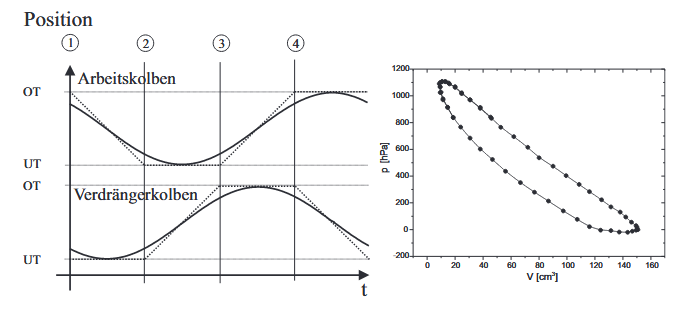
\includegraphics[width=0.9\textwidth]{graphics/einleitung/real.png}
    \caption{Realer Stirlingprozess; links: kontinuierliche Bewegung der Kolben, rechts: pV-Diagramm [Quelle: PAP2.1 Skript, S.38, 11.03.2024]}
    \label{fig:realStirling}
\end{figure}

\newpage
\subsubsection{Betrieb des Heißluftmotors als Kältemaschine oder Wärmepumpe}

Wir wollen nun betrachten, wie genau sich die Energiebilanz des Heißluftmotors aufstellen lässt, wenn man diesen als Kältemaschine betreibt. Die folgenden Rechnungen gelten im Umkehrschluss mit negativem Vorzeichen für den Fall der Wärmepumpe. Als Kältemaschine wird dem Motor pro Zyklus die Wärme $Q_2$ aus dem Zylinder entzogen, wobei die Wärme $Q_1$ hinzugefügt wird. Für den Wärmefluss muss dabei die mechanische Arbeit $W_M$ aufgebracht werden. Betrachtet man den Motor als ideal so gilt somit $Q_1 = Q_2 + W_M$ und der Wirkungsgrad ergibt sich als:

\begin{equation}
    \eta = \frac{Q_2}{W_M}.
    \label{eq:Kältemaschine-eta}
\end{equation}

Bei unserem Aufbau sorgt eine Heizwendel für eine konstante Raumtemperatur im Zylinder bei laufendem Motor. Somit entspricht die von der Heizung pro Umlauf geleistete elektrische Arbeit $W_H$ genau der dem System zugeführten Wärme $Q_2$, die sich aus der Spannung und Stromstärke der Heizung $U_H \ \& \ I_H$ sowie der Drehzahl $f$ ergibt:

\begin{equation}
    Q_2 = W_H = \frac{U_H I_H}{f}.
    \label{eq:Kältemaschine-Q_2}
\end{equation}

Die vom Motor an die Kühlung abgegebene Wärme $Q_1$ kann mit der kalorischen Zustandsgleichung berechnet werden: 

\begin{equation}
    Q_1 = \frac{c_W \rho_W \Delta T  \dot{V}}{f}.
    \label{eq:Kältemaschine-Q_1}
\end{equation}

Hierbei stehen $c_W$ und $\rho_W$ für die Wärmekapazität sowie die Dichte von Wasser und $\Delta T = T_{zu} - T_{ab}$ und $\dot{V}$ für die Temperaturdifferenz des Zu- und Abflusses beziehungsweise den Volumenstrom des Kühlwassers.

Zuletzt lässt sich noch die pro Zyklus zugeführte mechanische Arbeit $W_M$ aus Strom und Spannung des Antriebsmotors berechnen:

\begin{equation}
    W_M = \frac{U_M I_M}{f}.
    \label{eq:Kältemaschine-W_M}
\end{equation}


\subsubsection{Betrieb des Heißluftmotors als Wärmekraftmaschine}

Beim Betrieb als Wärmekraftmaschine wird der Motor mit einer elektrischen Heizwendel durch die zugeführte elektrische Energie $Q_{el}$ beheizt. Da insgesamt bei sowohl der Beheizung als auch der Wärmeabstrahlung und -leitung viel Energie verloren geht, muss der Teil des Verlust $Q_v$ berücksichtigt werden. Es wird also effektiv nur die Wärme $Q_{el} - Q_v$ in das System geführt. 

Teilweise wird diese Wärme in die mechanische Arbeit $W_{mech}$ umgewandelt, welche sich einmal durch Berechnung der Fläche des zugehörigen pV-Diagramms und andererseits durch eine Drehmomentmessung bestimmen lässt. Bei letzterem wird ein Pronyscher Bremszaum verwendet, welcher eine variable Bremskraft auf die Motorwelle ausübt, zu sehen in Abbildung \ref{fig:Bremsbalken}. Misst man dabei mit einem Kraftmesser am Ende des waagrerechten Bremszaums senkrecht die wirkende Kraft $F$, so ergibt sich das Drehmoment $D$:

\begin{equation}
    D = l F.
\end{equation}

Die Länge $l$ bezeichnet dabei die Länge vom Aufhängepunkt des Kraftmessers bis zur Motorachse. Man erhält somit die pro Zyklus abgebene Arbeit $W_D$ und Leistung $P_D$:

\begin{equation}
    \begin{split}
        W_D &= 2 \pi D = 2 \pi l F, \\
        P_D &= W_D f = 2 \pi l F f.
    \end{split}
    \label{eq:Wärmekraftmaschine-W_D&P_D}
\end{equation}

Erneut bezeichnet $f$ hierbei die Drehzahl des Motors. Für die gesamte Energiebilanz müssen nun noch die ungenutzte Abwärme $Q_{ab}$ sowie die Reibungsverluste $Q_R$ berücksichtigt werden und man erhält:

\begin{equation}
    Q_el = Q_v + W_{mech} + Q_{ab} + Q_R.
    \label{eq:Wärmekraftmaschine-Energiebilanz}
\end{equation}

Insgesamt kann man die Verluste nicht direkt bestimmen, sondern diese nur abschätzen. Für den gesamten Verlust $Q_V$ gilt:

\begin{equation}
    Q_V = Q_v + Q_R = Q_{el} - Q_{ab} - W_{mech}.
    \label{eq:Wärmekraftmaschine-Verlust}
\end{equation}

Die pro Zyklus zugeführte Wärme $Q_{el}$ wird erneut aus der elektrischen Heizleistung $P_{el}$ und der Motordrehzahl $f$ bestimmt, während die ans Kühlwasser abgegebene Wärme $Q_{ab}$ wieder aus der kalorischen Zustandsgleichung hervorgeht:

\begin{equation}
    Q_{el} = \frac{P_{el}}{f} = \frac{U I}{f},
    \label{eq:Wärmekraftmaschine-Q_el}
\end{equation}

\begin{equation}
    Q_{ab} = \frac{c_W \rho_W \Delta T  \dot{V}}{f}.
    \label{eq:Wärmekraftmaschine-Q_ab}
\end{equation}

\begin{figure}[!b]
    \centering
    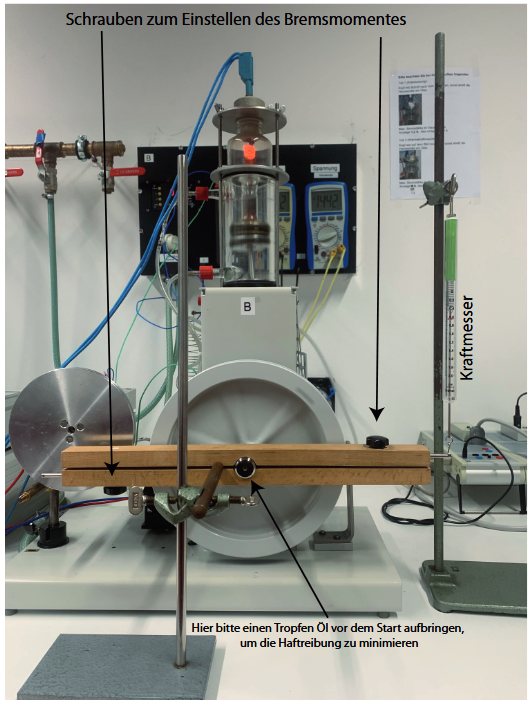
\includegraphics[width=0.55\textwidth]{graphics/einleitung/bremse.png}
    \caption{Drehmomentmessung an der Motorwelle [Quelle: PAP2.1 Skript, S.44, 11.03.2024]}
    \label{fig:Bremsbalken}
\end{figure}


\clearpage
\newpage
\subsection{Versuchsaufbau}

\subsubsection{Aufbau des Heißluftmotors}

Wir verwenden einen $\beta$-Typ Heißluftmotor wie in den Grundlagen erklärt. In Abbildung \ref{fig:aufbau} sowie der Skizze auf der ersten Seite des Messprotokolls sind die genaueren Aspekte des Aufbaus dargestellt. Am Aufbau können wir die folgenden Werte messen:

\begin{itemize}
    \item[-] Zu- und Abflusstemperatur sowie Durchlussmenge des Kühlwassers.
    \item[-] Druck und Volumen im Zylinder des Motors
    \item[-] Spannung und Stromstärke des Antriebmotors
    \item[-] Spannung und Stromstärke des Heizelements
    \item[-] Motordrehzahl
    \item[-] Senkrechte Kraft auf den Bremsblock
    \item[-] Je nach Zylinderaufsatz:
        \begin{itemize}
            \item Temperatur im oberen Teil des Motorzylinders
            \item Temperatur der sich im Reagenzglas befindeten Flüssigkeit
        \end{itemize}
\end{itemize}

Dabei gibt es, wie nun schon vorweggenommen, verschiedene Zylinderköpfe, die auf den Motor geschraubt werden können. Der im ersten Teil verwendete Zylinderkopf besitzt eine Heizwendel sowie ein eingebautes Thermometer, der zweite ein Reagenzglas, in welches ein zusätzlicher Temperaturfühler eingelassen werden kann, und der Dritte besitzt nur eine Heizwendel.

Die Antriebsmotor- und Heizleistungen können jeweils über einen Drehregler eingestellt werden. Wird im letzten Teil der Bremszaum verwendet, so kann man diesen über die Schrauben zwischen den Blöcken zu- beziehungsweise aufdrehen und somit die effektive Bremskraft regulieren, welche dann am Kraftmesser abgelesen wird. 

\subsubsection{Verwendete Messsoftware}

Zusätzlich dienen zur Messung noch die Programme 'Thermolink' und 'CASSY-LAB'. Ersteres zeichnet die von den ans gleichnamige Thermoelemt angeschlossenen Thermoelemente über einen längeren Zeitraum auf und kann somit die Verläufe abspeichern. Hier werden vor allem die Temperaturen des Kühlwassers sowie des Zylinderkopfs im ersten Teil beobachtet. 

Mit CASSY-LAB können zum einen der im zweiten Teil verwendete Temperaturfühler im Reagenzglaus und zum anderen die Daten des im letzten Teil genutzten Druck- und Volumenmessers aufgezeichnet werden. Dabei kann aus Letzteren sofort das pV-Diagramm gebildet und dessen Fläche vom Programm berechnet werden.

\begin{figure}[!b]
    \centering
    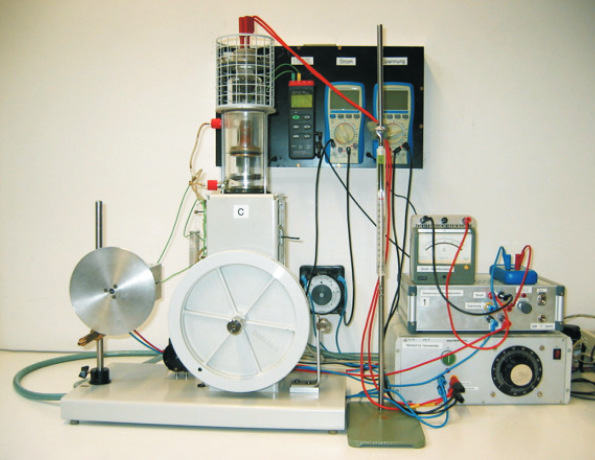
\includegraphics[width=0.9\textwidth]{graphics/einleitung/versuchsaufbau.png}
    \caption{Übersicht des Versuchsaufbaus [Quelle: PAP2.1 Skript, S.33, 11.03.2024]}
    \label{fig:aufbau}
\end{figure}


%---------------VERSUCHSPROTOKOLL MIT MESSDATEN---------------
\newpage

\section{Versuchsprotokoll mit Messdaten}

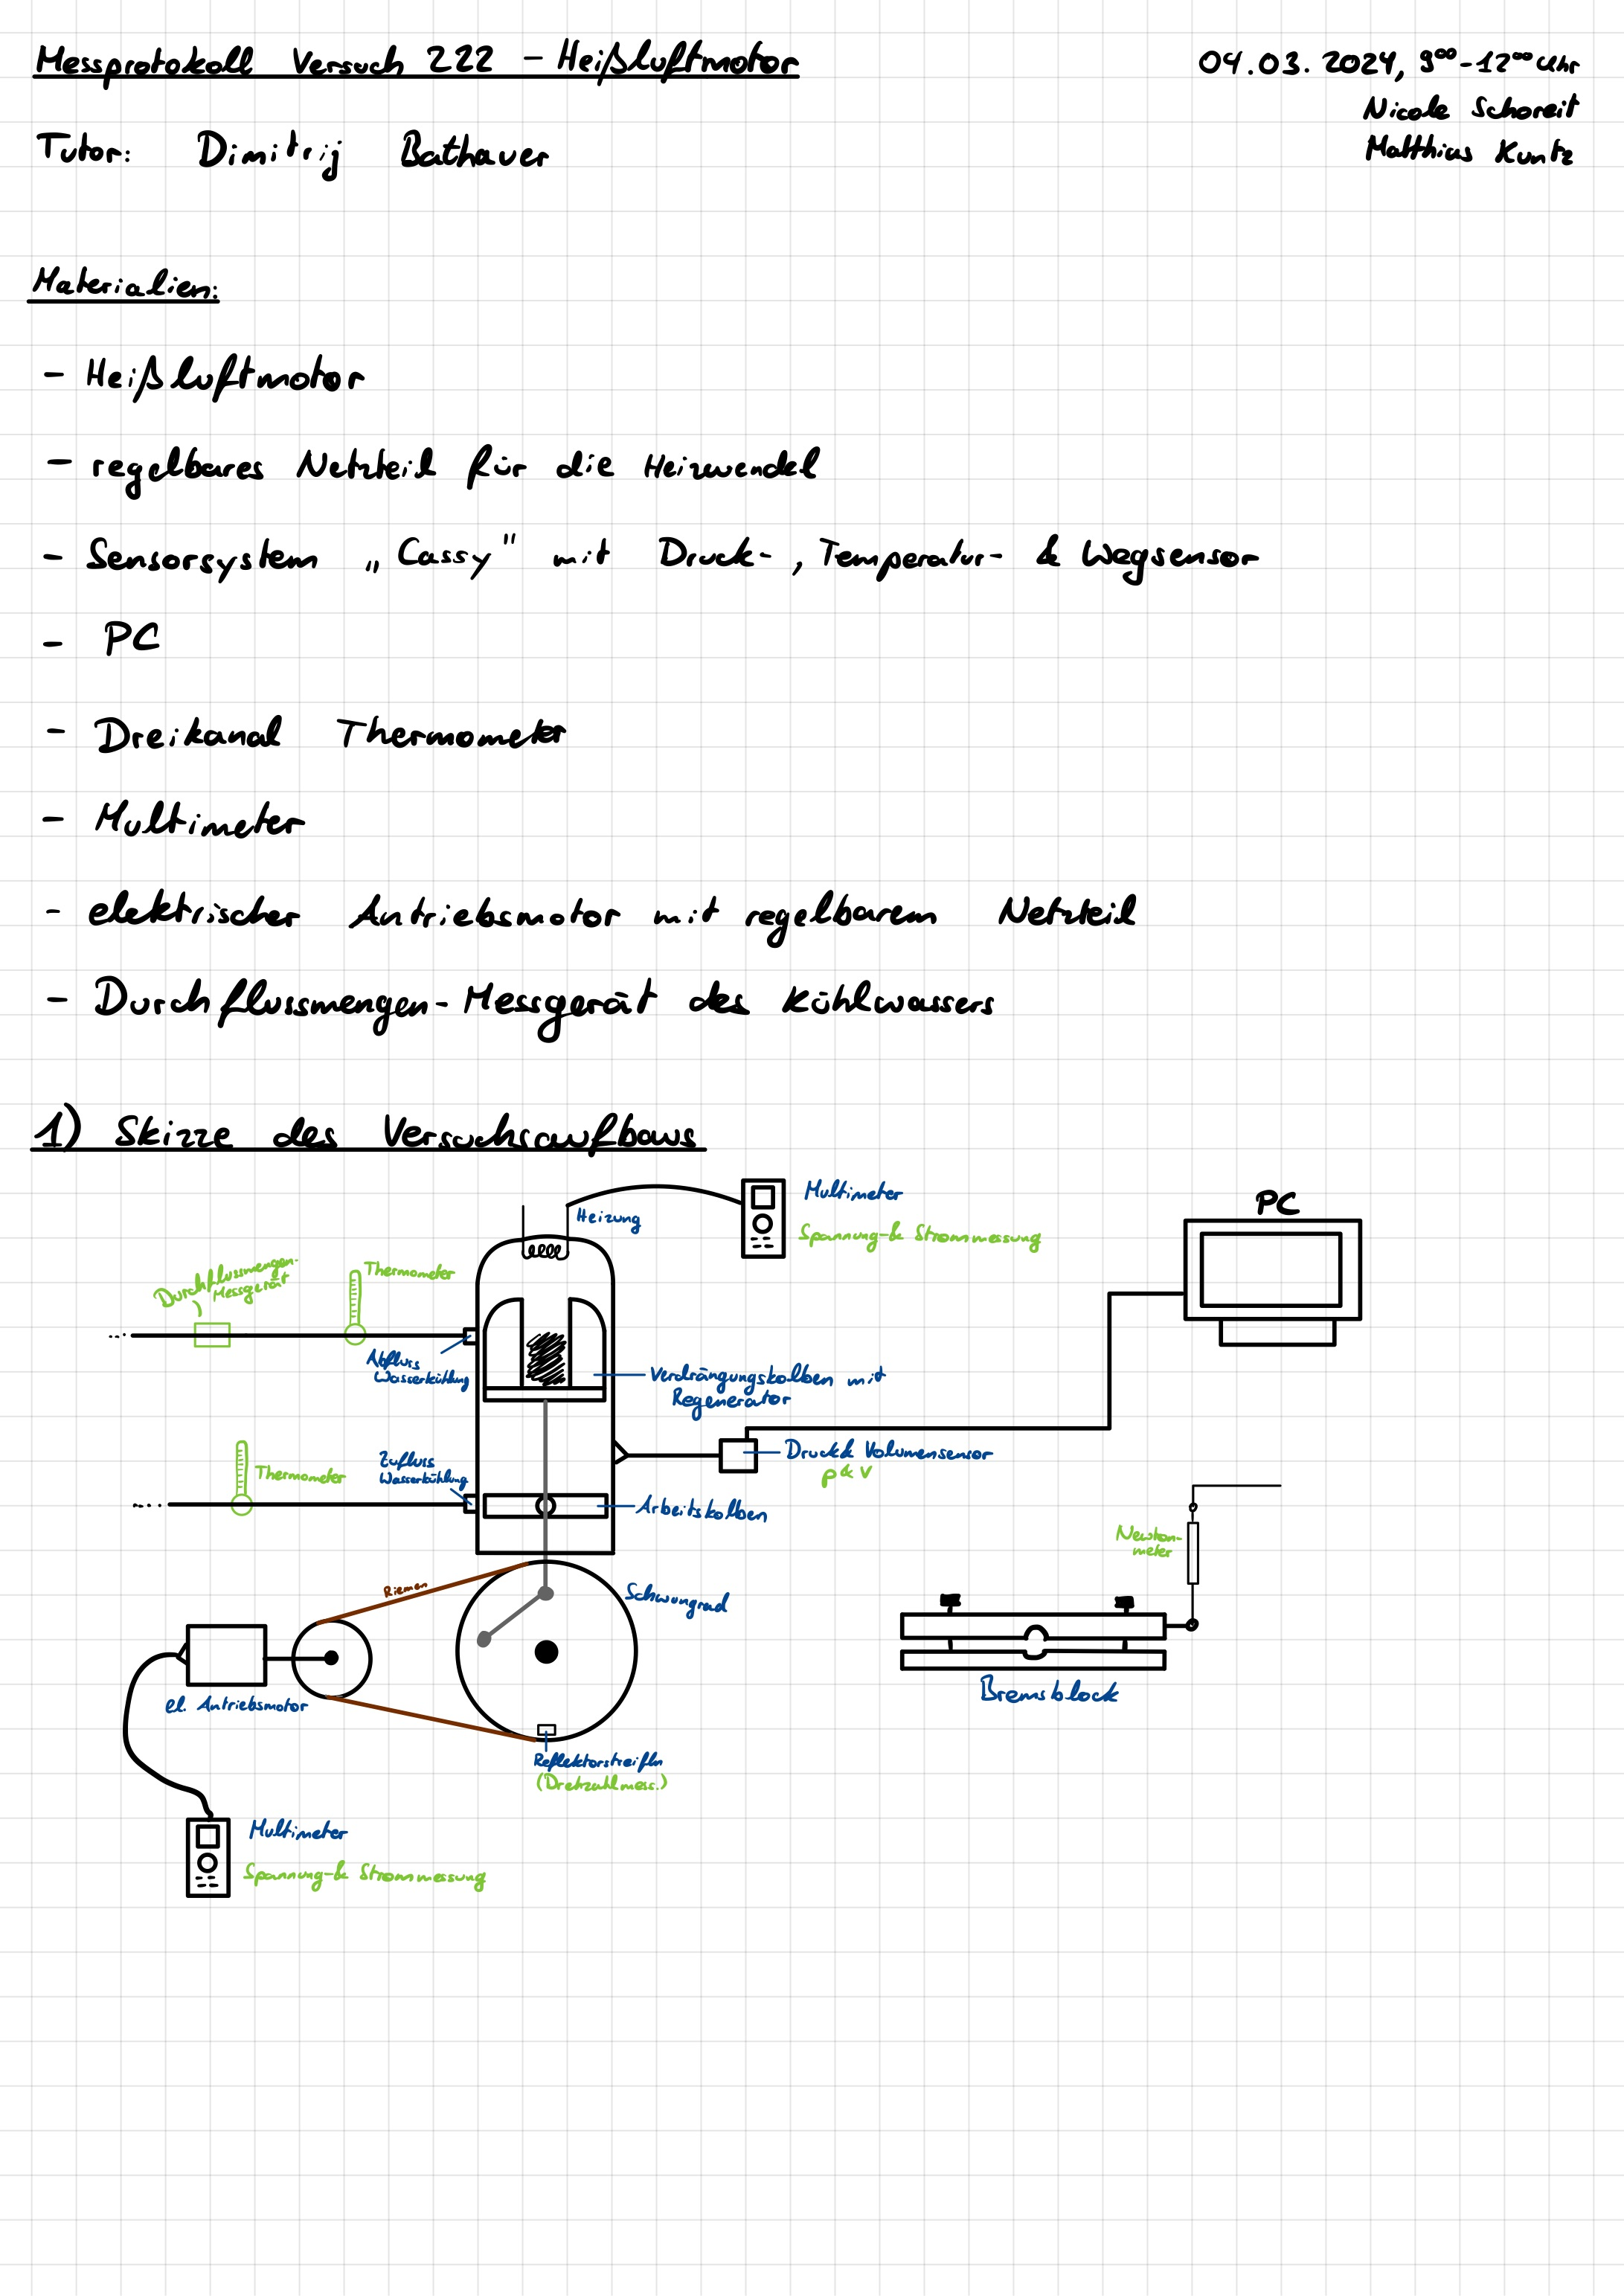
\includegraphics[width=\textwidth]{graphics/mess1.jpg}
\newpage
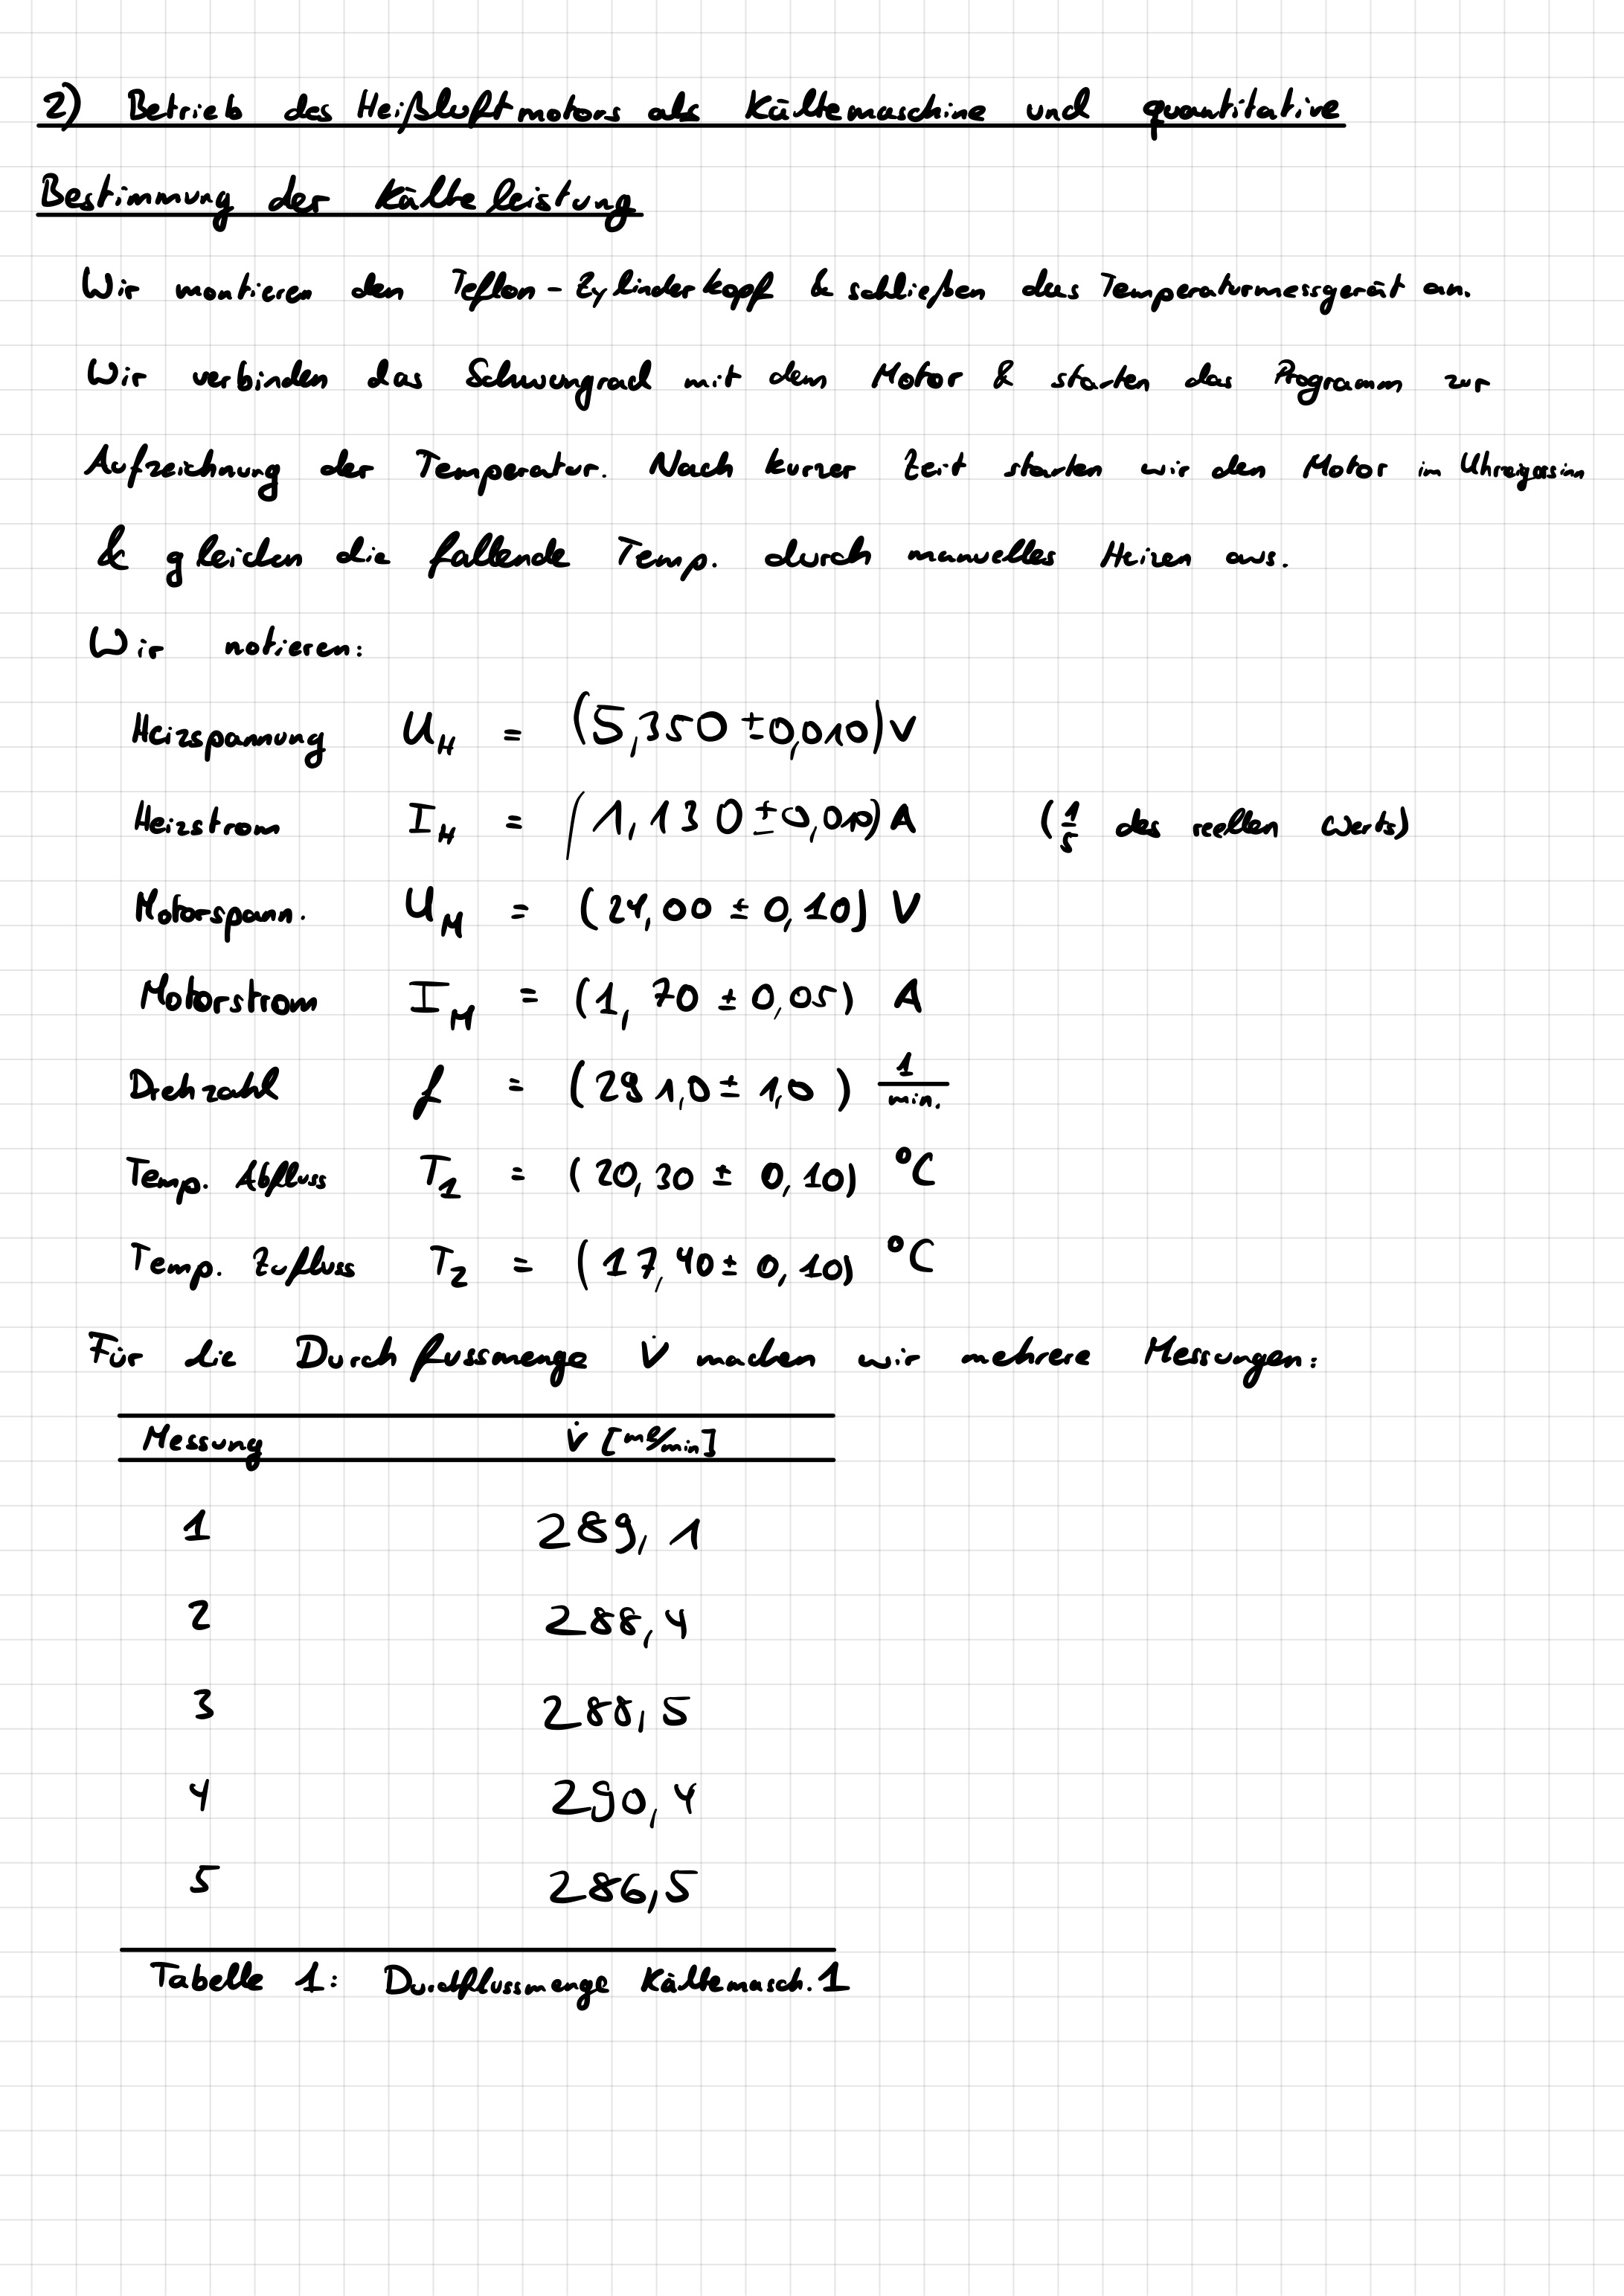
\includegraphics[width=\textwidth]{graphics/mess2.jpg}
\newpage
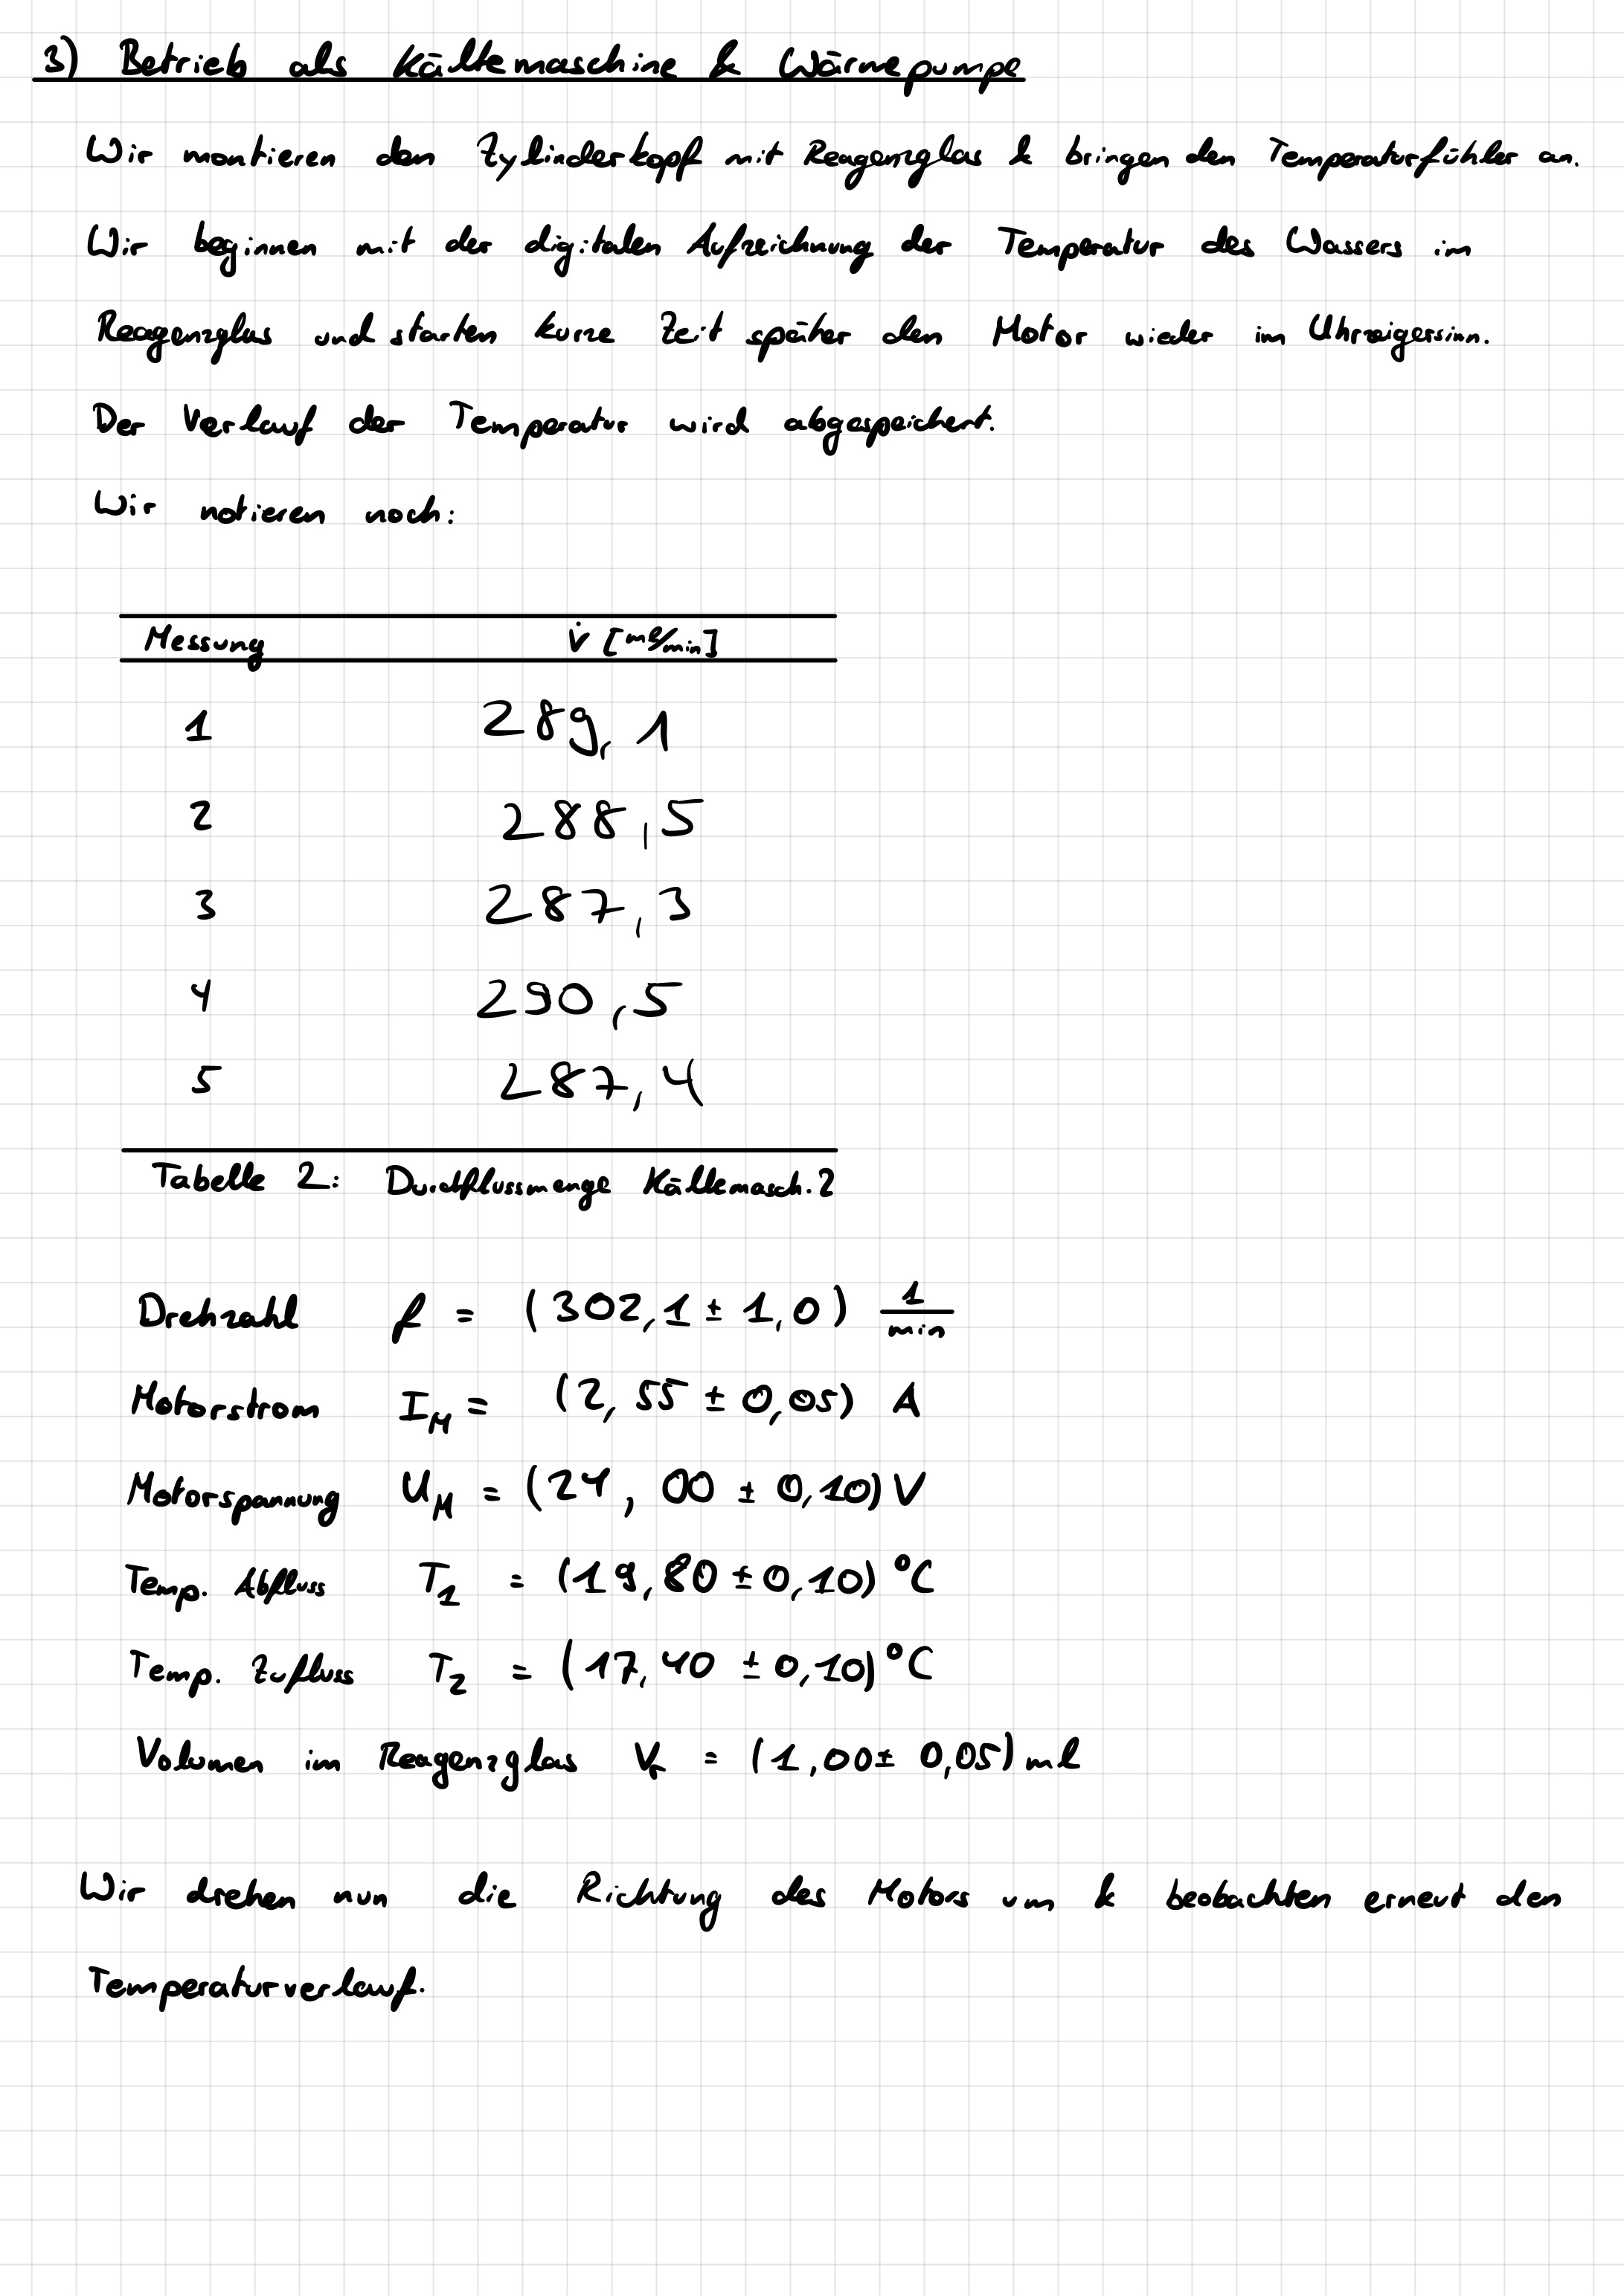
\includegraphics[width=\textwidth]{graphics/mess3.jpg}
\newpage
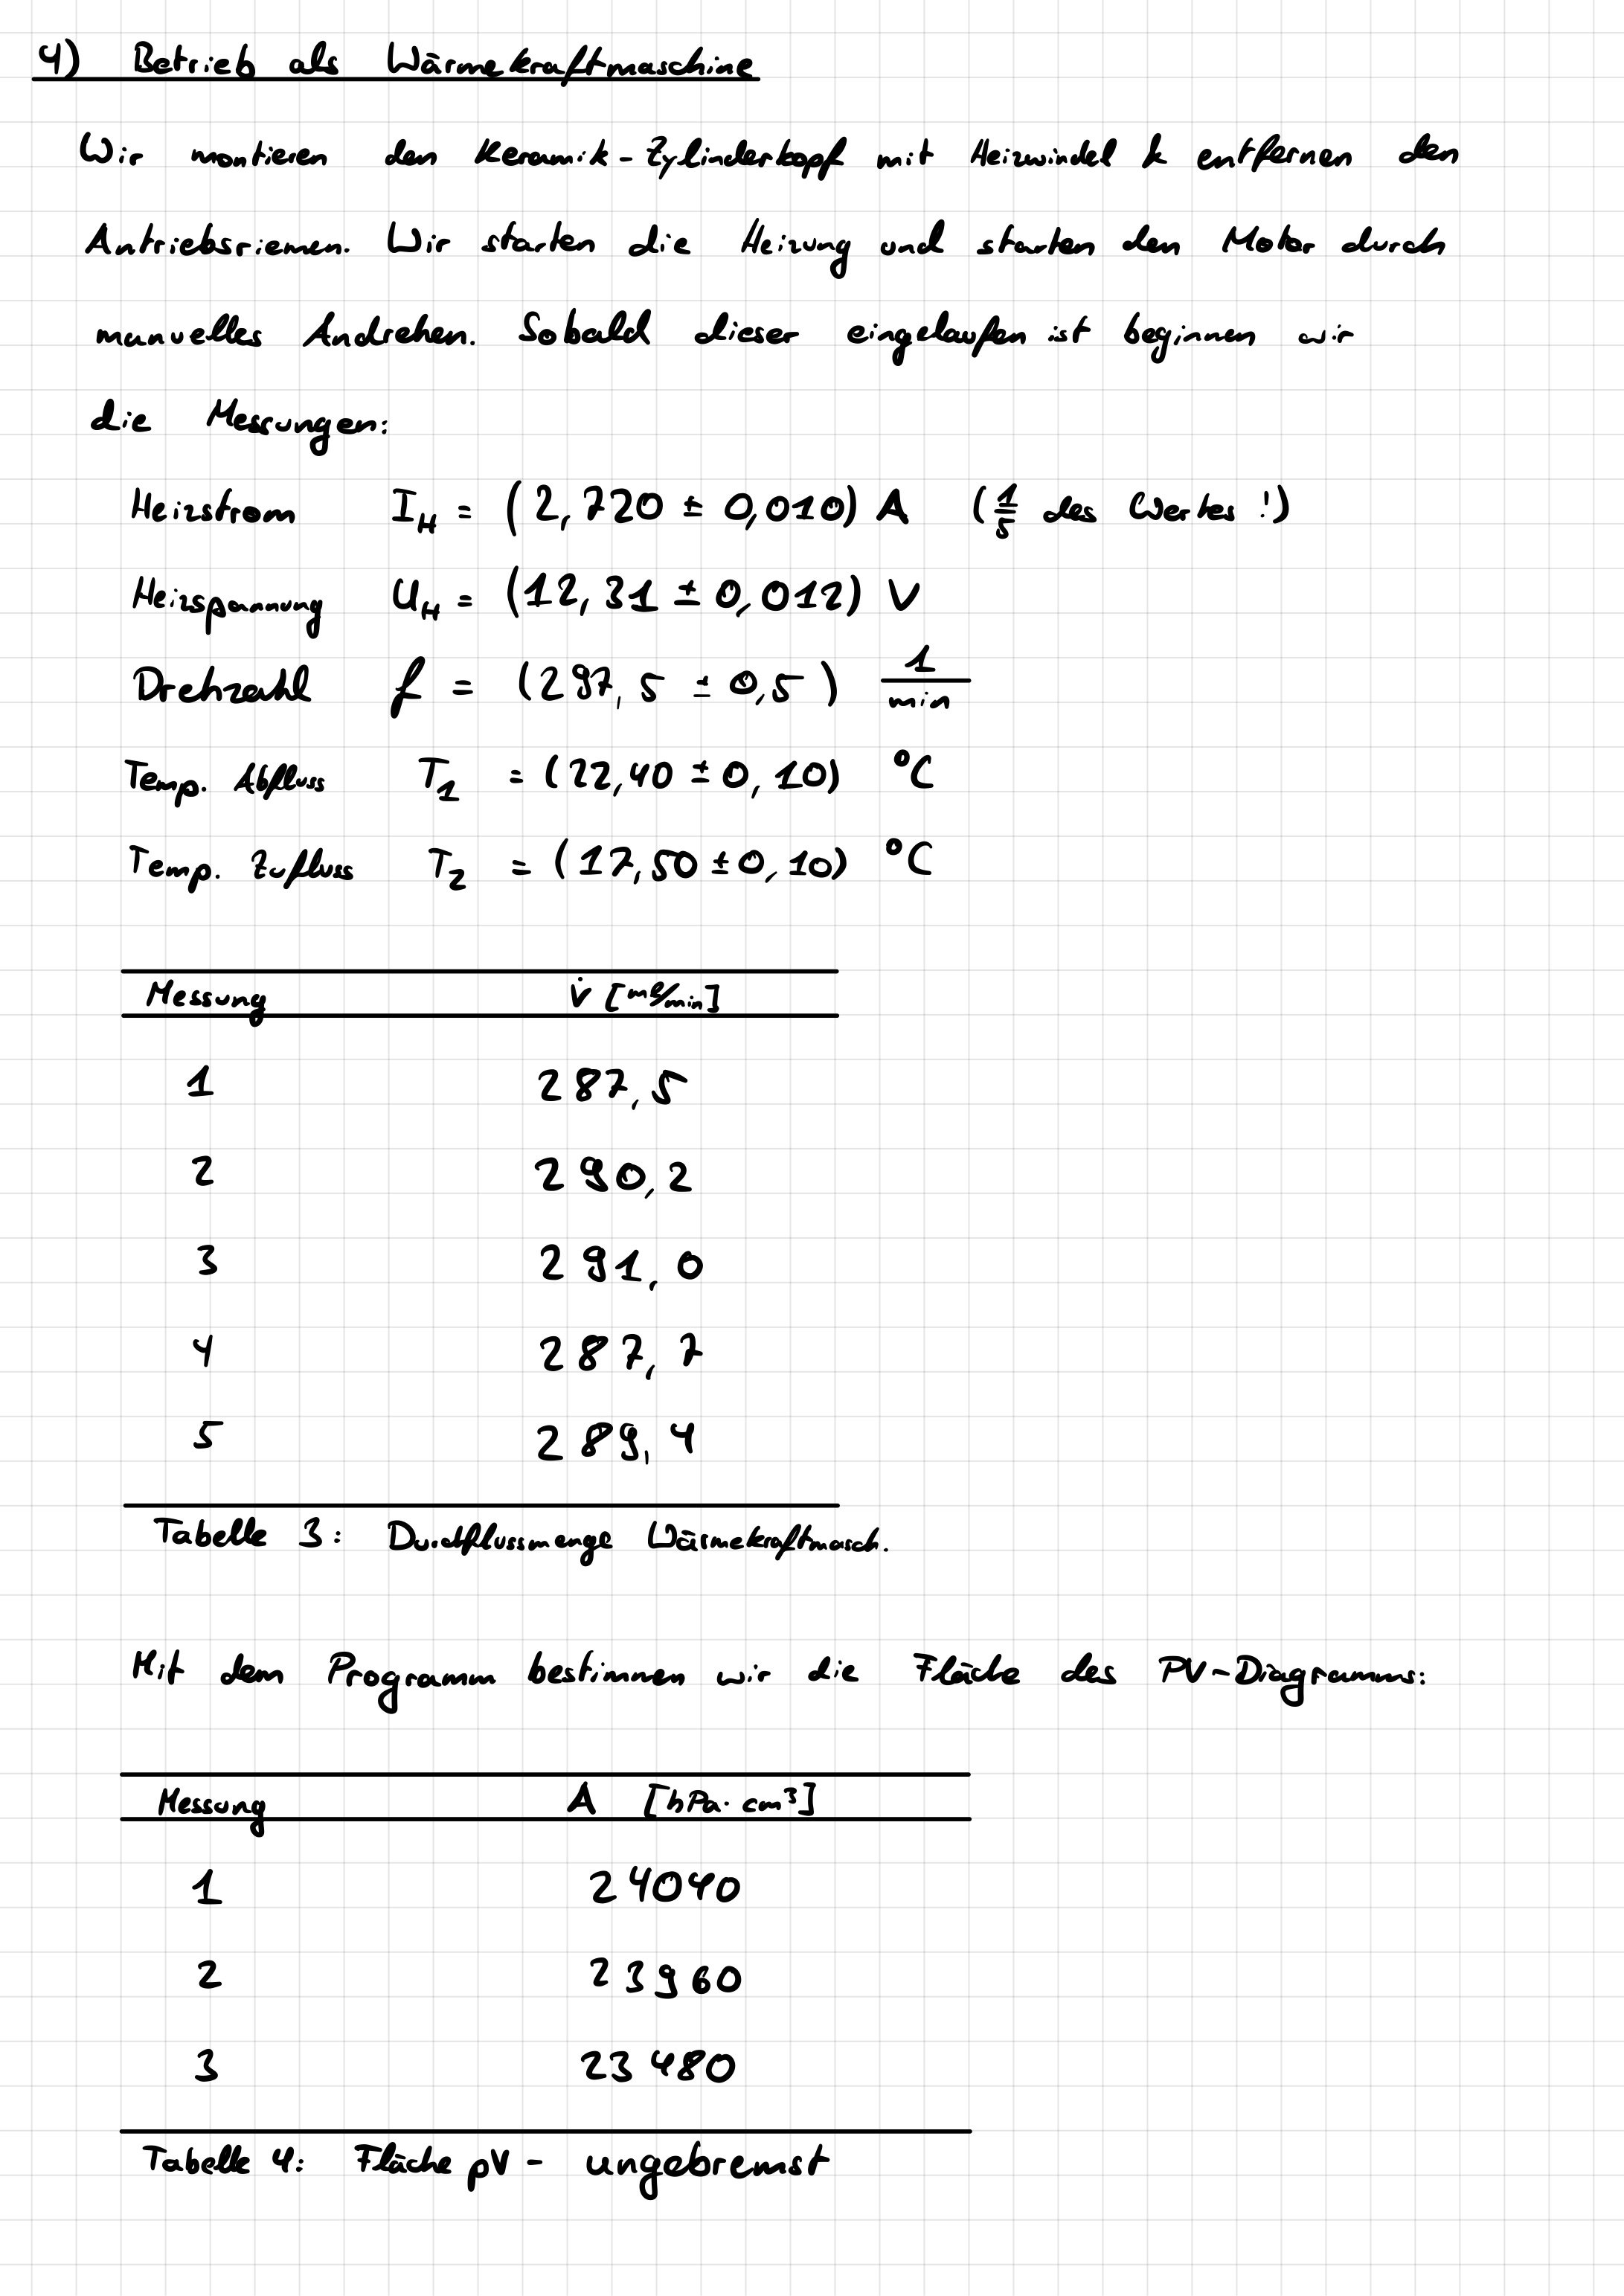
\includegraphics[width=\textwidth]{graphics/mess4.jpg}
\newpage
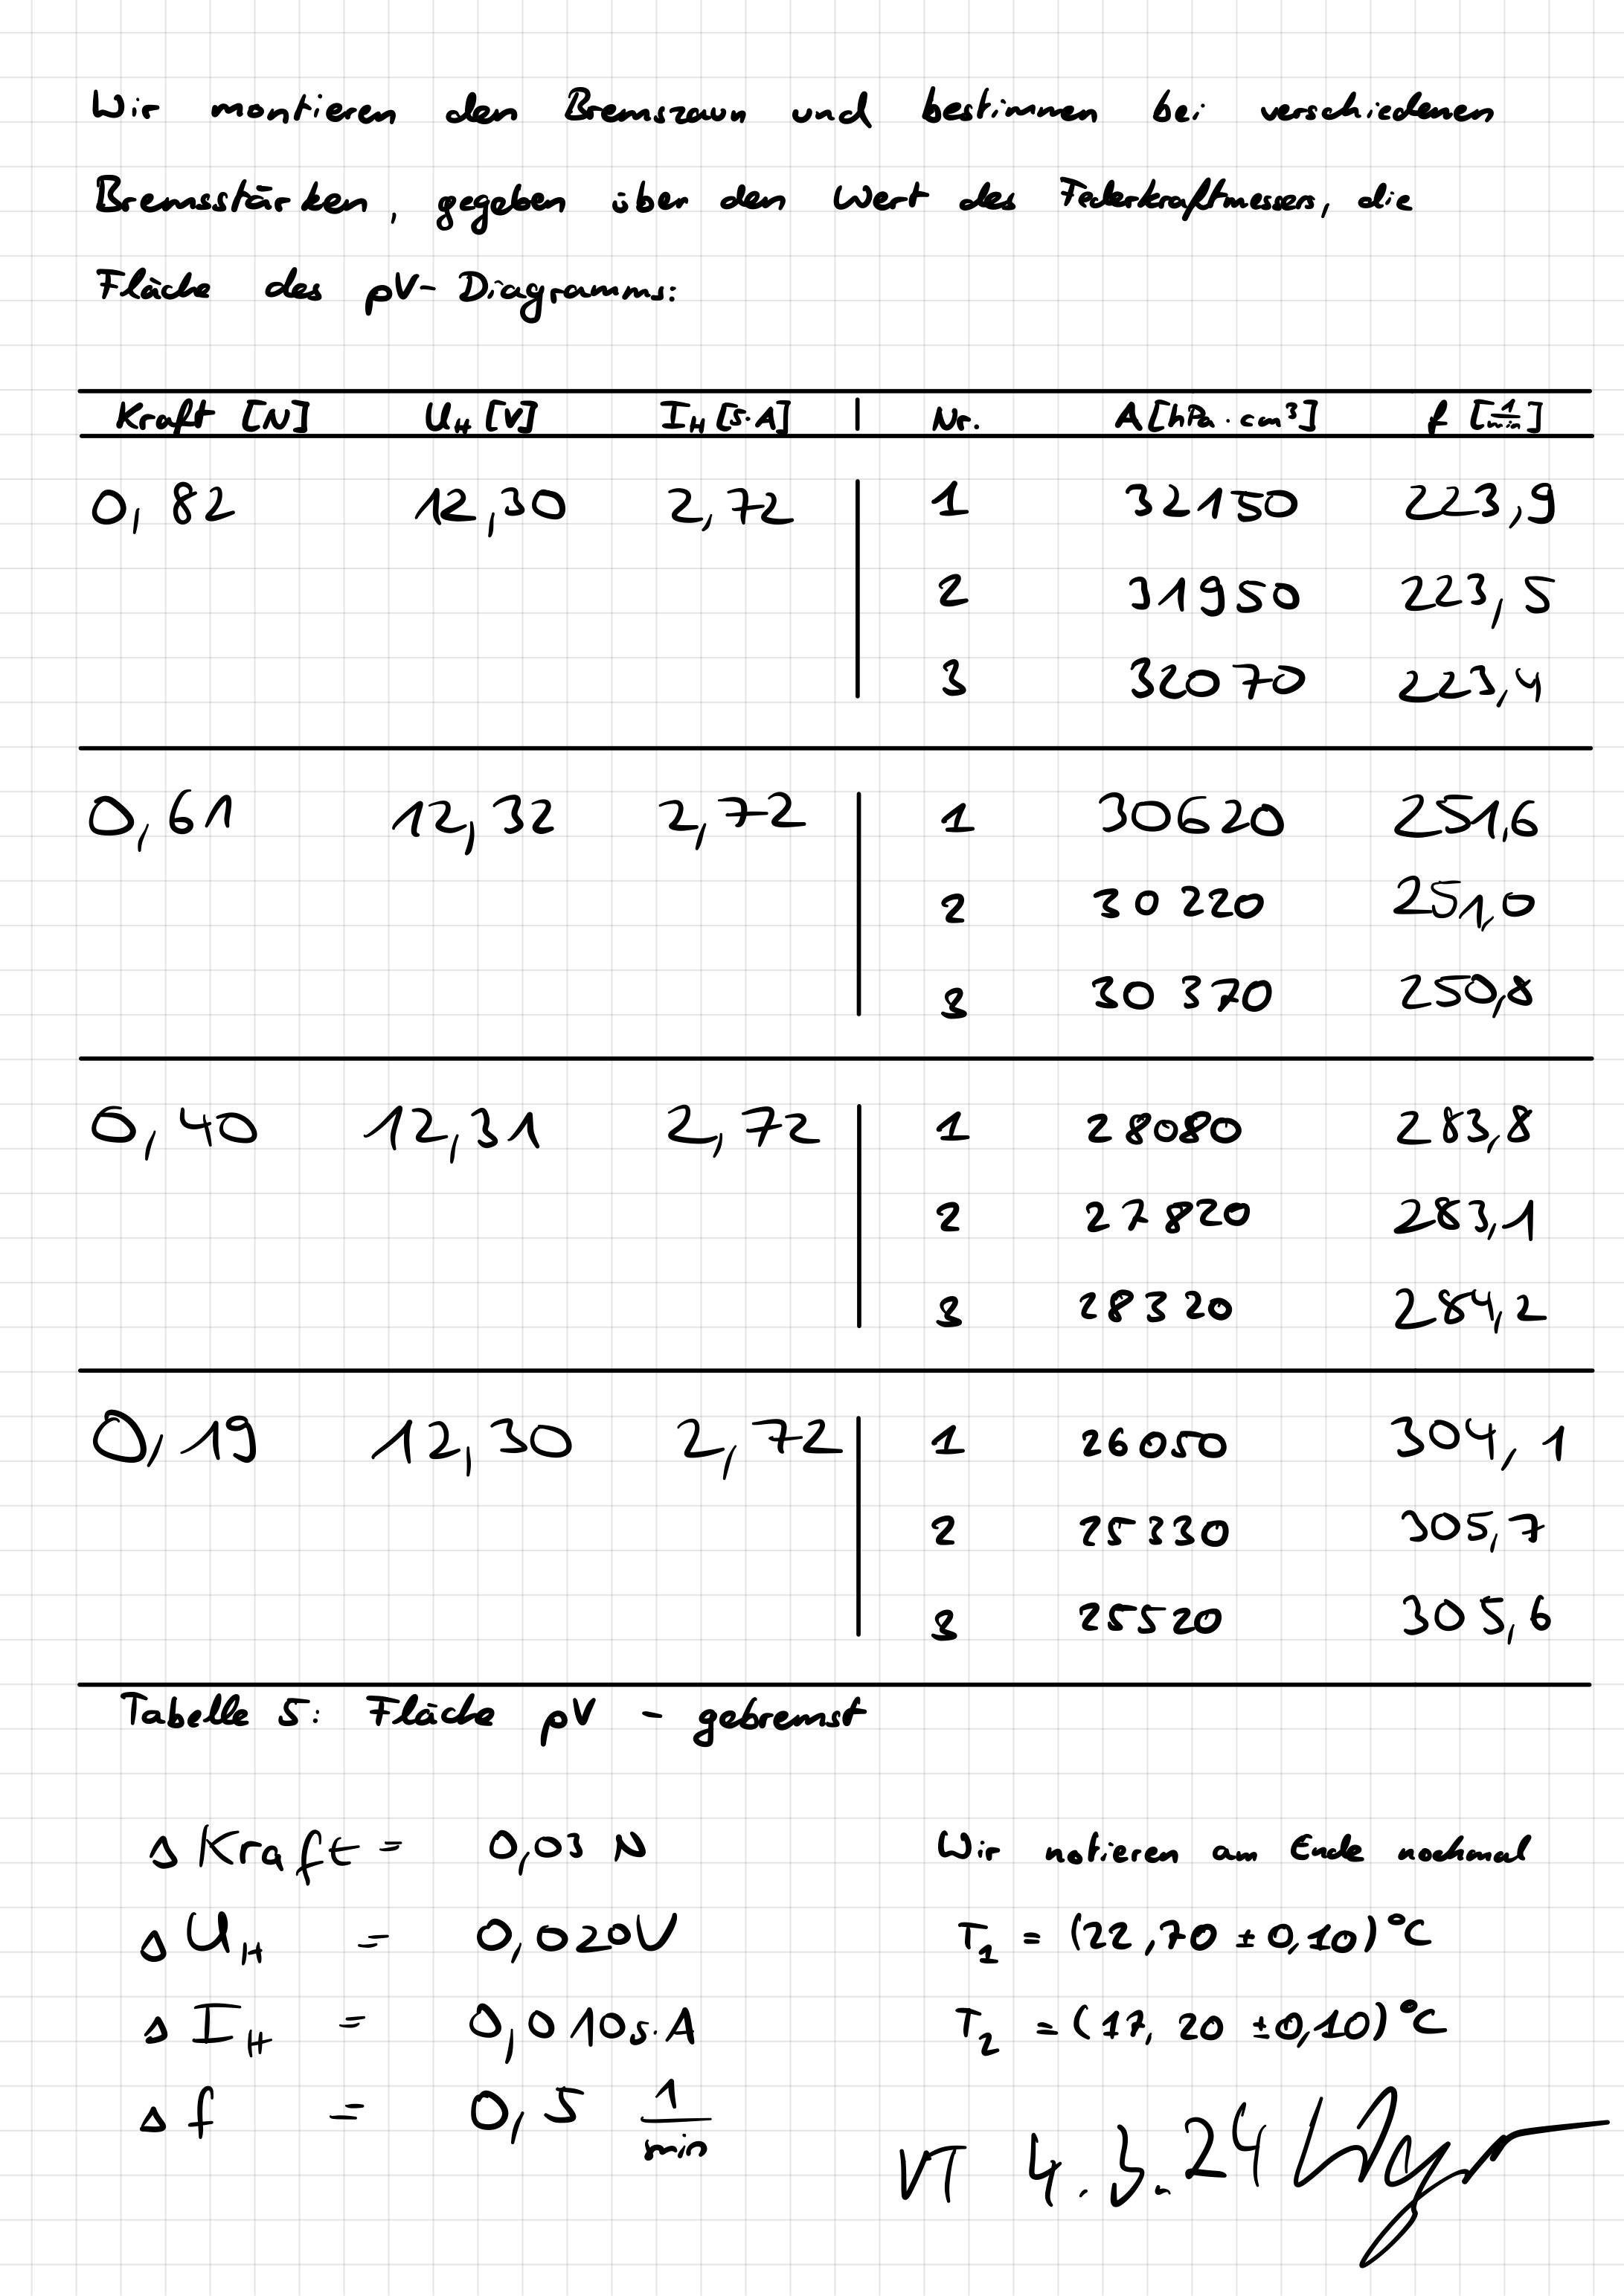
\includegraphics[width=\textwidth]{graphics/mess5.jpg}
\newpage

\addtocounter{table}{5}

\begin{figure}[!p]
    \centering
    \resizebox{0.9\textwidth}{!}{
    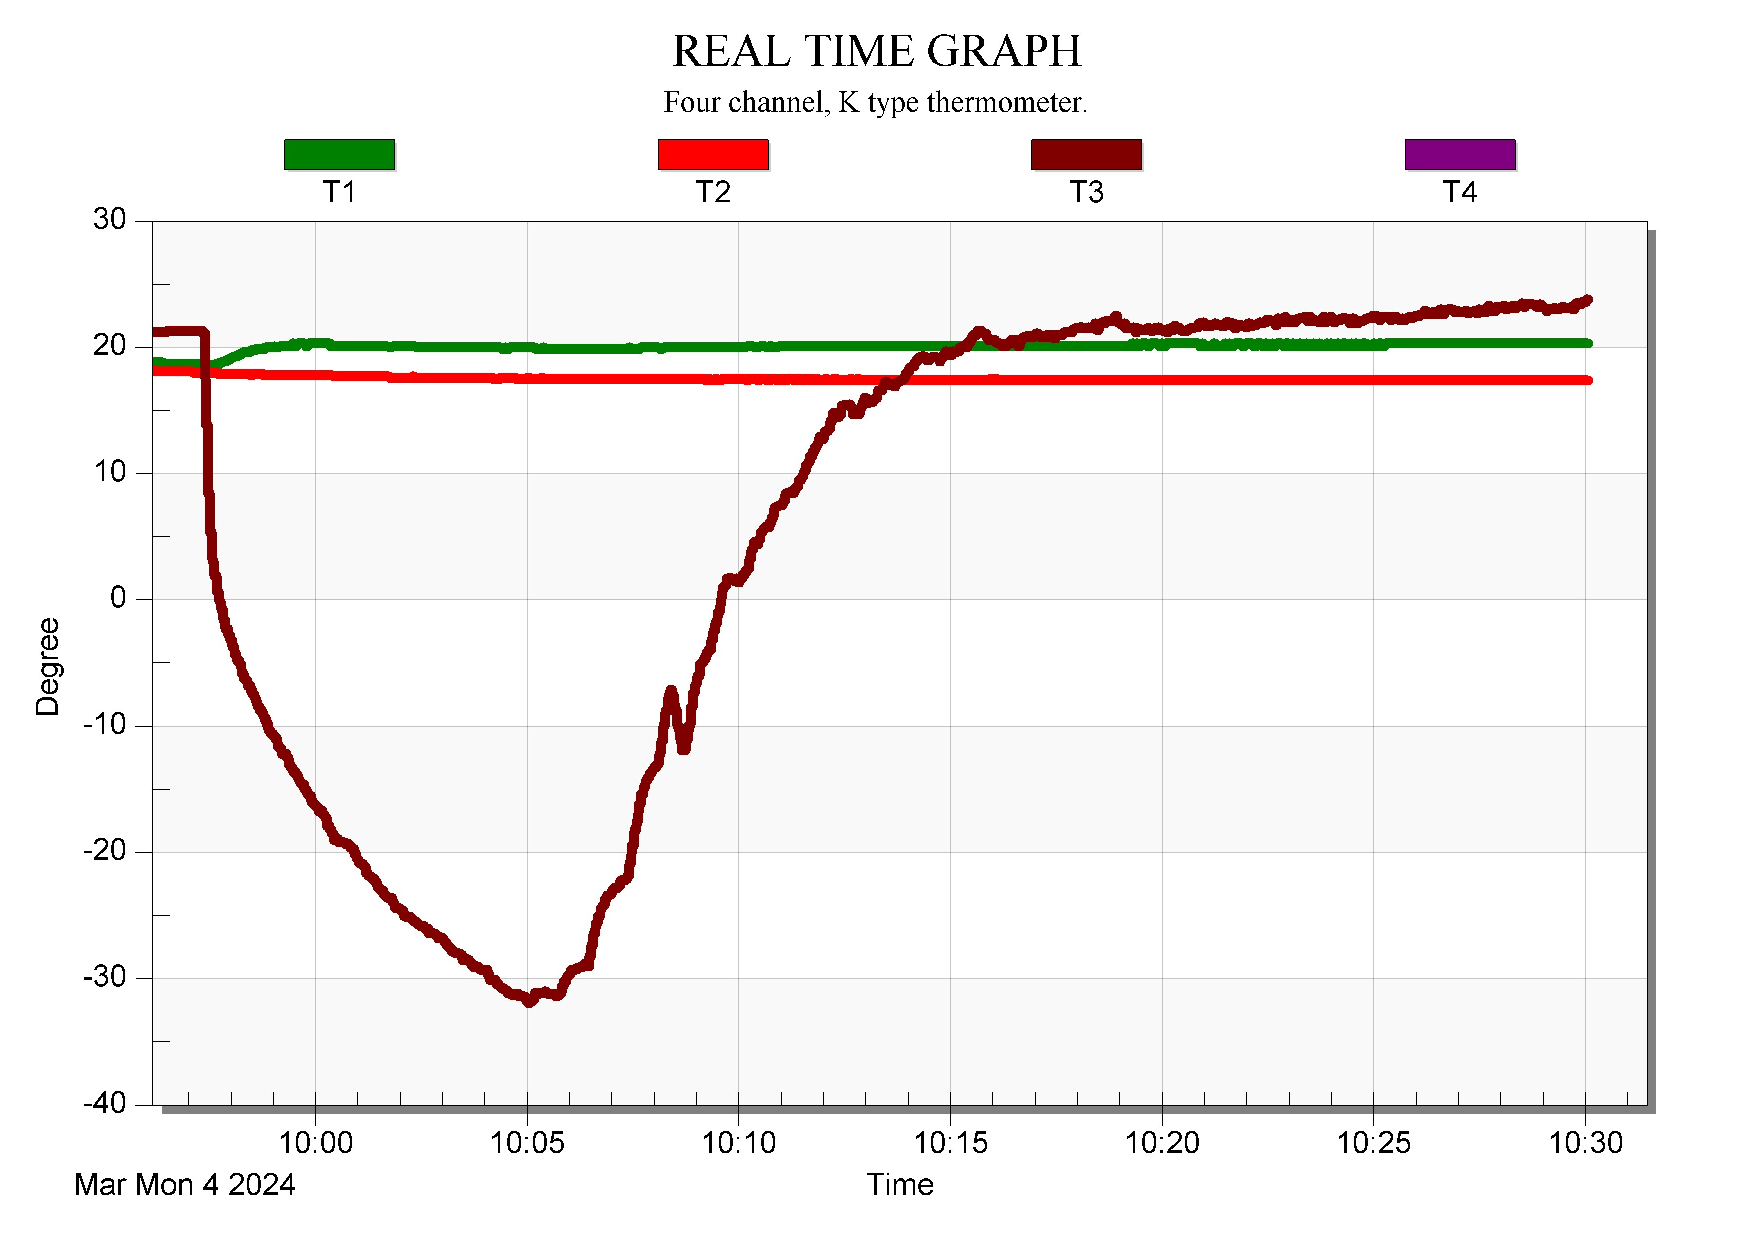
\includegraphics{graphics/messungen/temp A2.pdf}}
    \caption{Temperaturverlauf bei Teil 2: \\ T1=Abfluss Kühlung; T2=Zufluss Kühlung; T3=Temp. im Zylinder}
    \label{fig:temp2}
\end{figure}

\begin{figure}[!p]
    \centering
    \resizebox{\textwidth}{!}{
    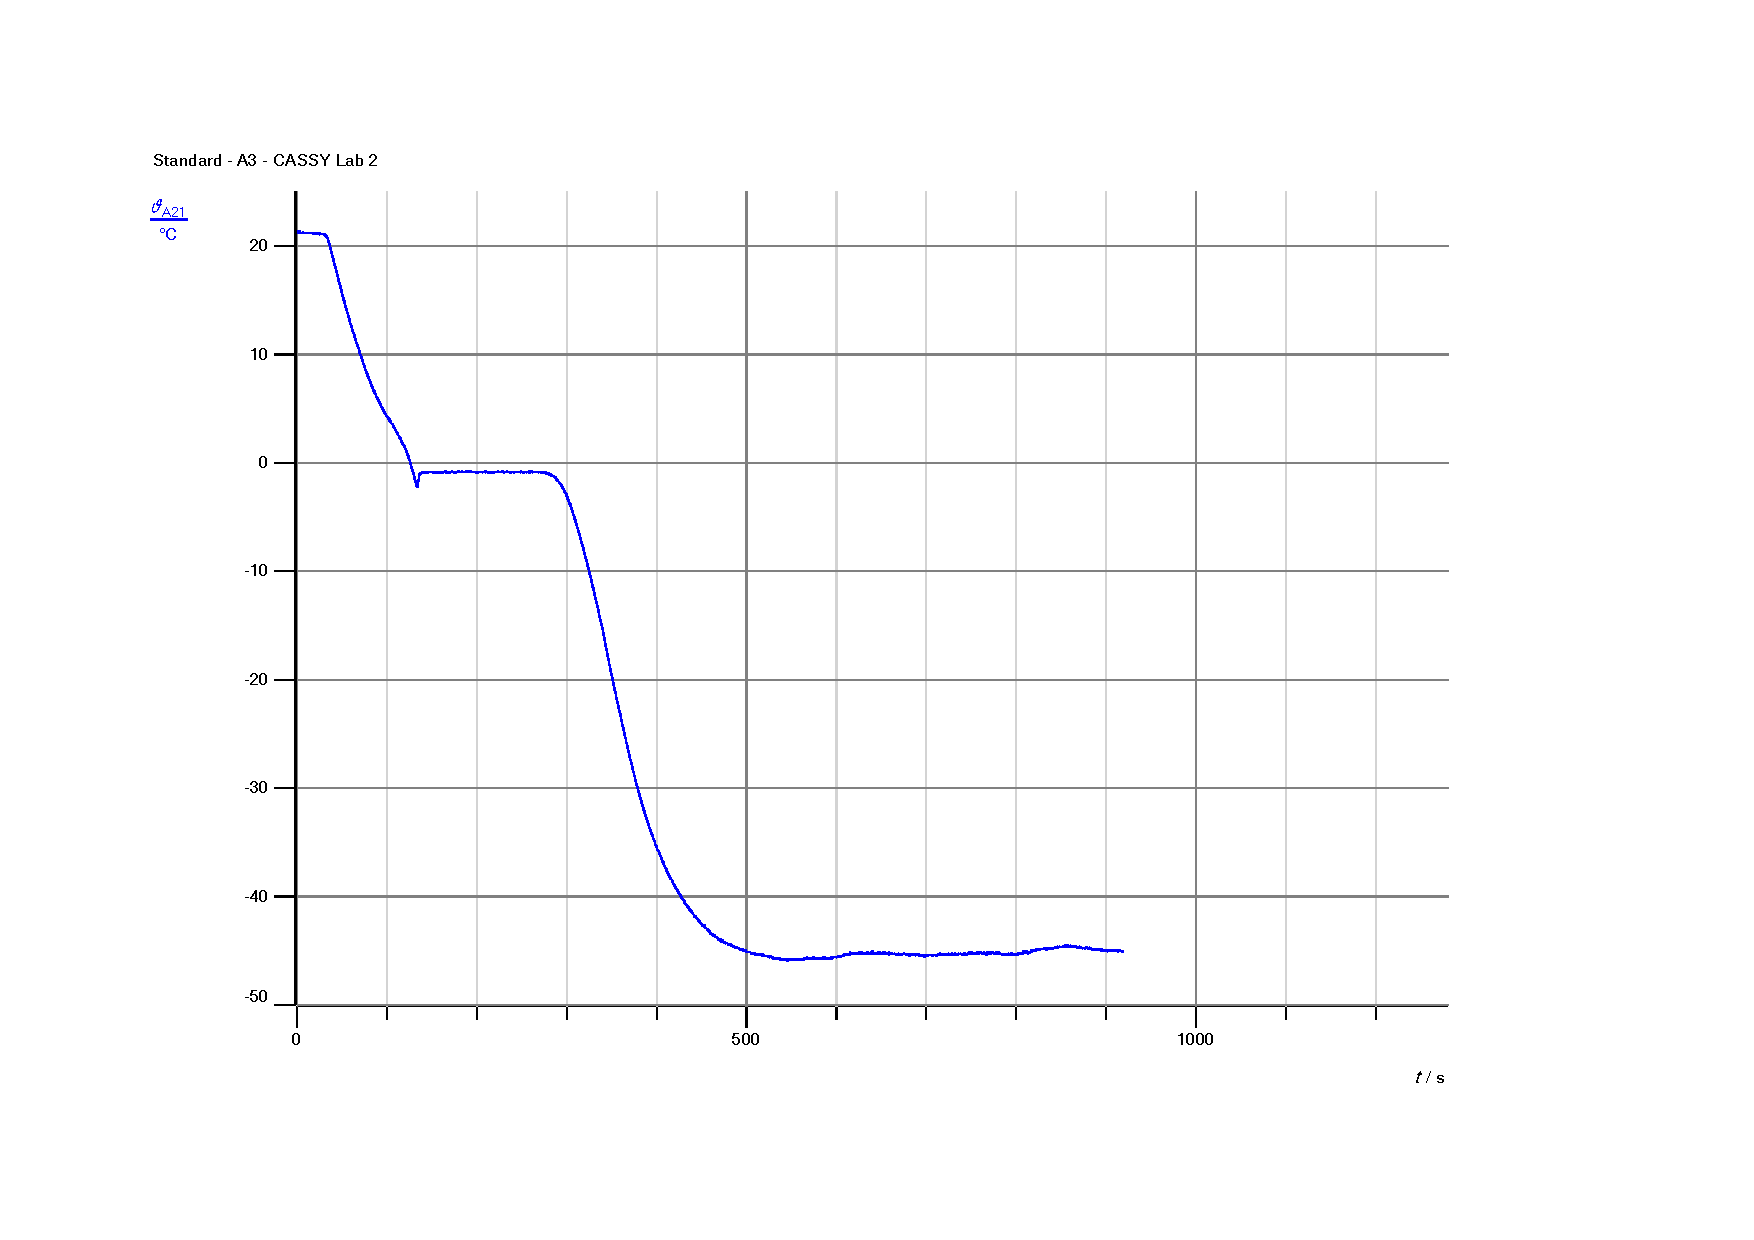
\includegraphics{graphics/messungen/A3 1.pdf}}
    \caption{Temperaturverlauf des Wassers bei Teil 3: Kältemaschine - Gesamte Messung}
    \label{fig:temp31-ges}
\end{figure}

\begin{figure}[!p]
    \centering
    \resizebox{\textwidth}{!}{
    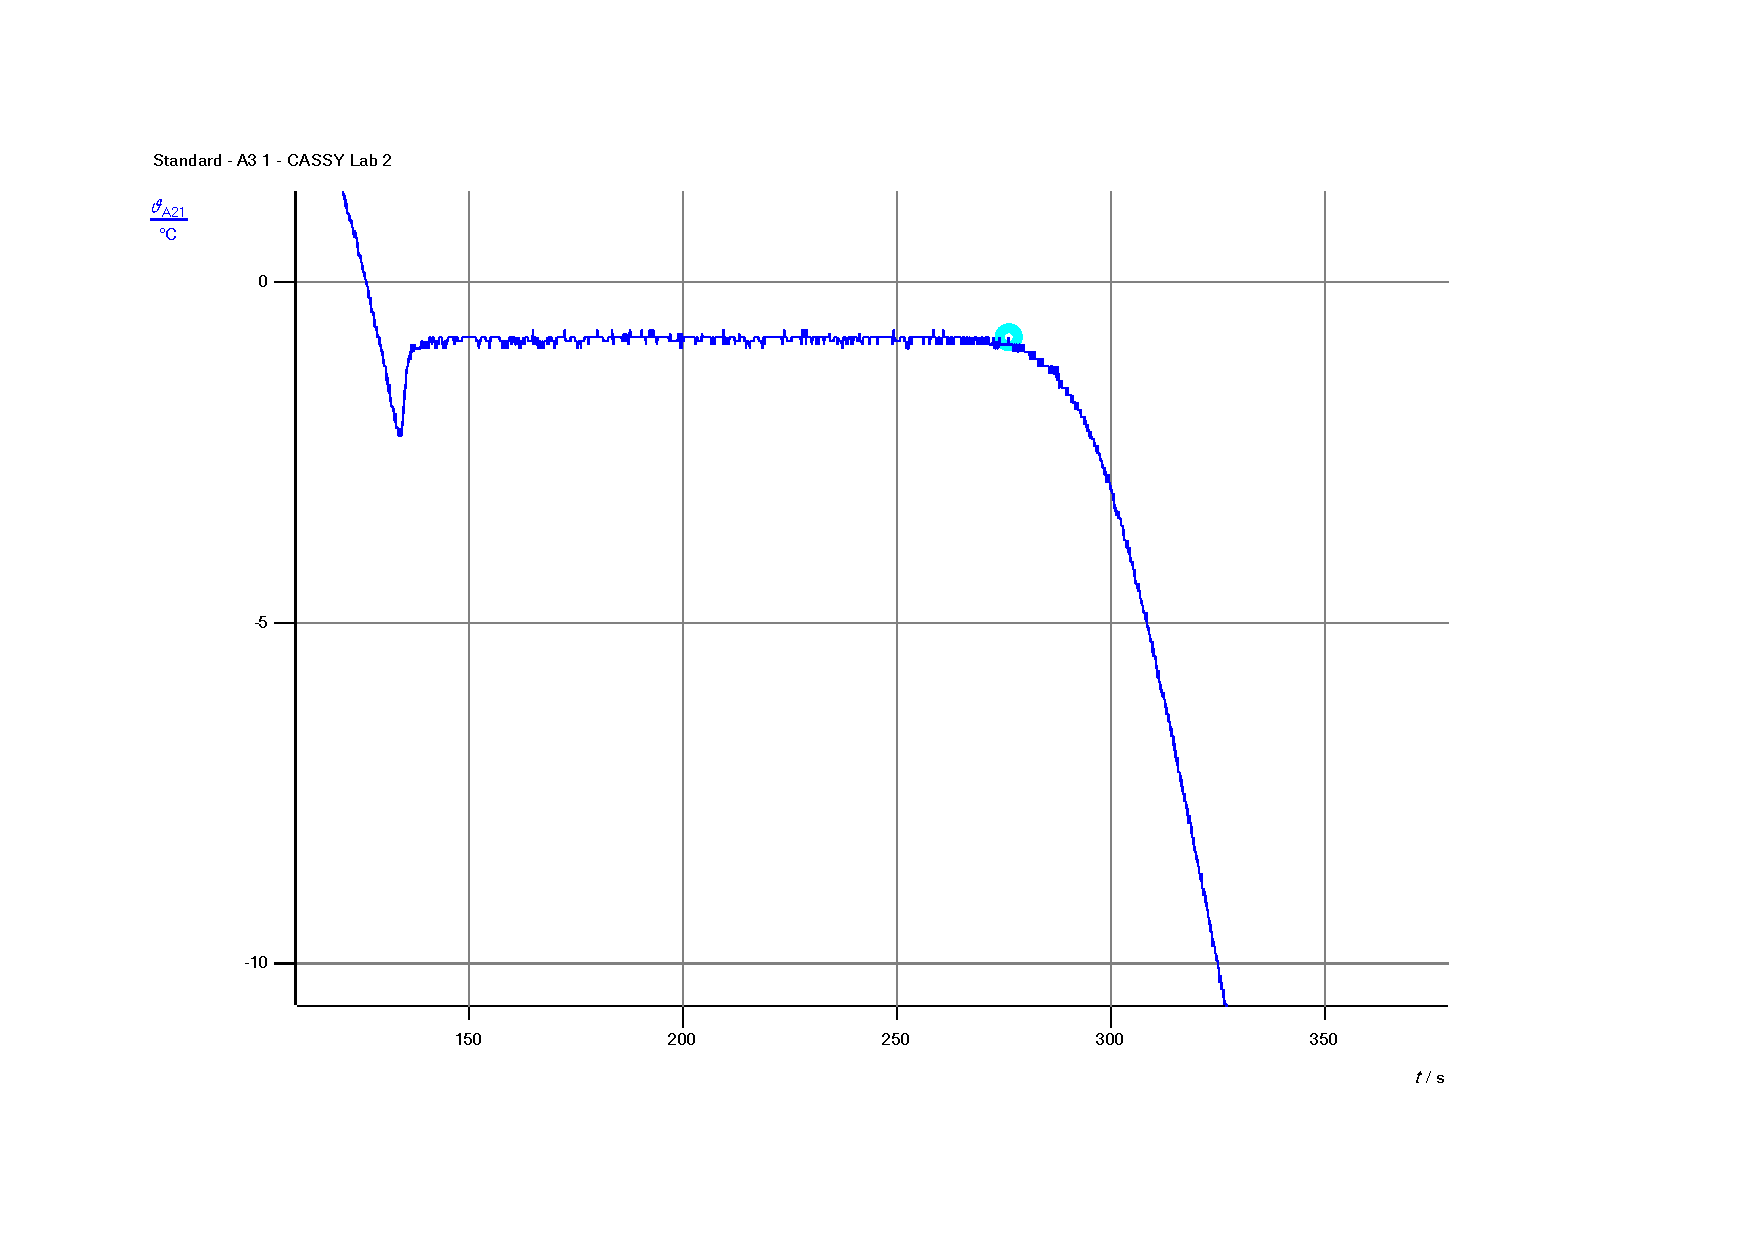
\includegraphics{graphics/messungen/A3 1 zoom gerade.pdf}}
    \caption{Temperaturverlauf des Wassers bei Teil 3: Kältemaschine - Zoom auf Gefrierprozess}
    \label{fig:temp31-zoom}
\end{figure}

\begin{figure}[!p]
    \centering
    \resizebox{\textwidth}{!}{
    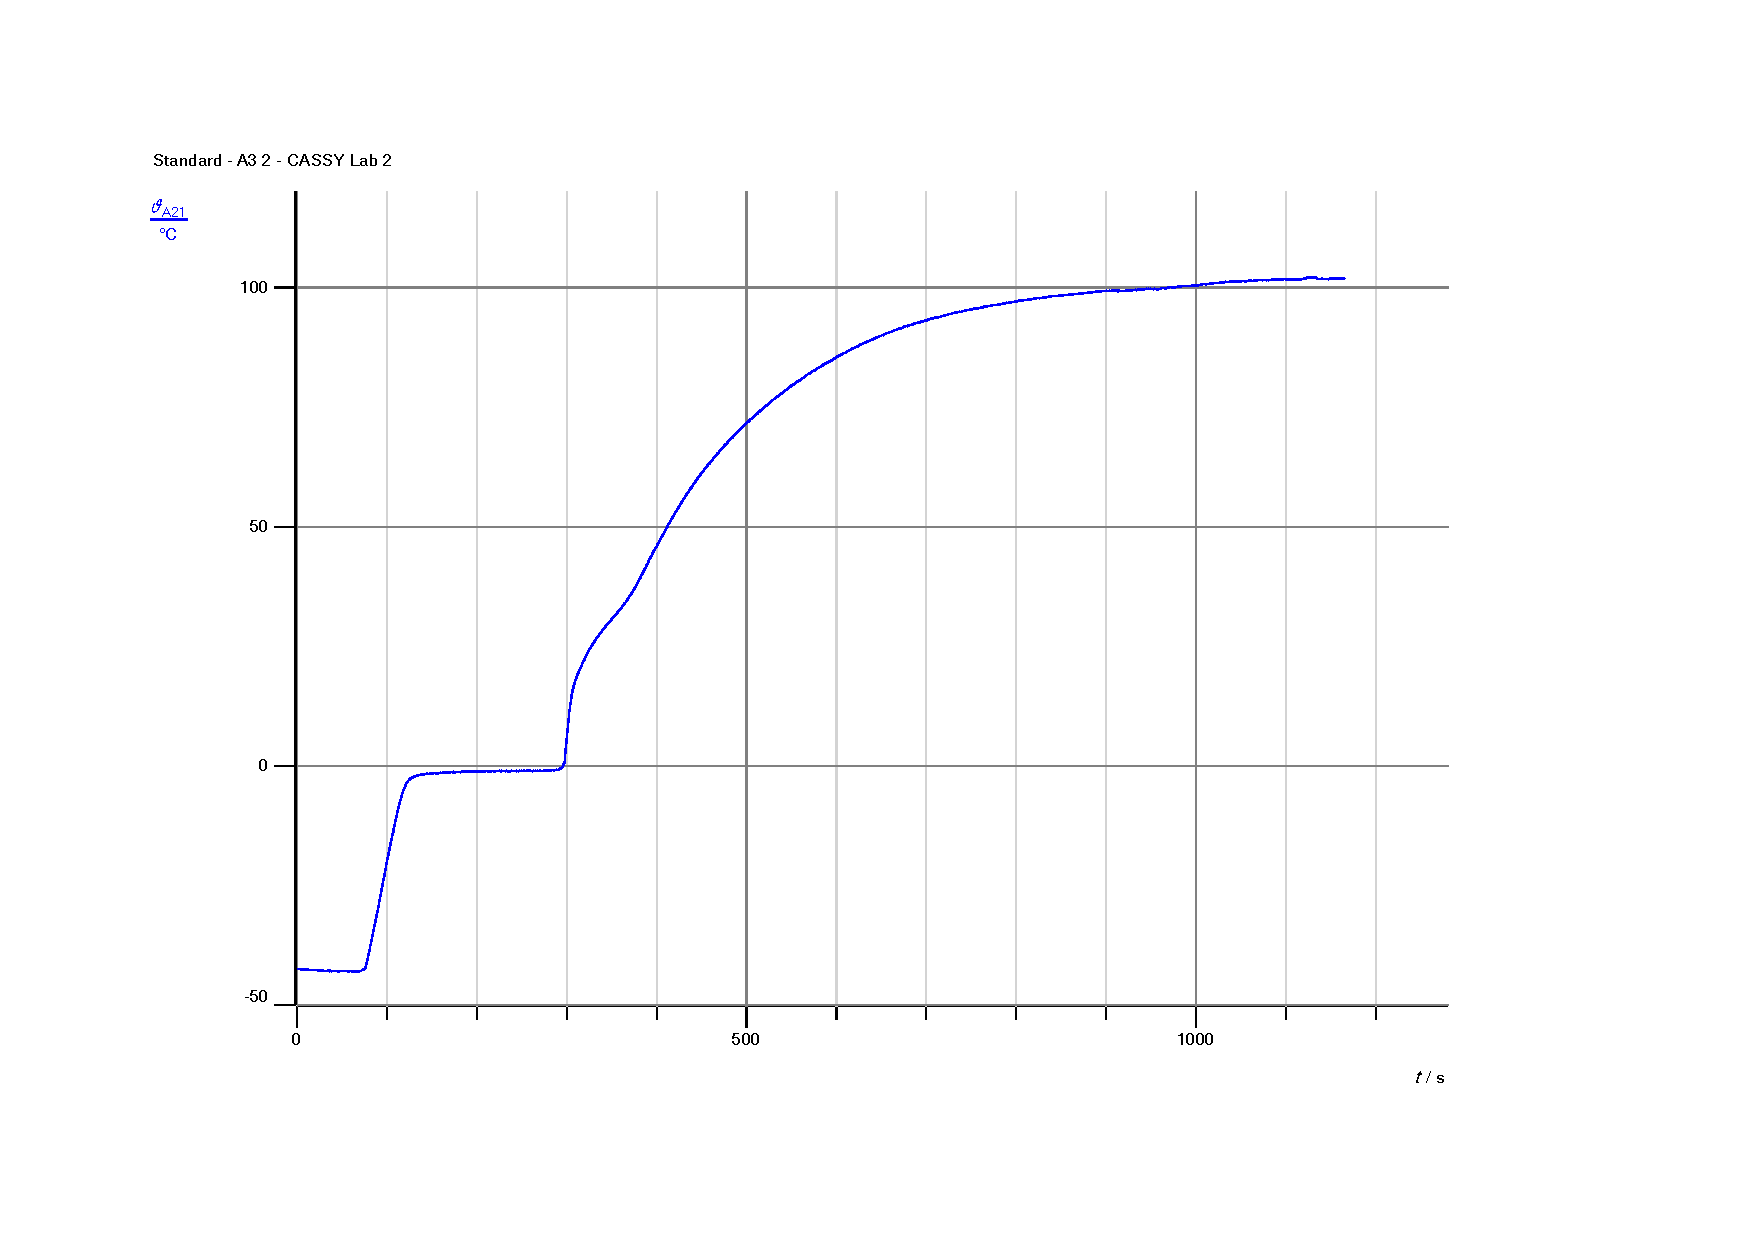
\includegraphics{graphics/messungen/A3 22.pdf}}
    \caption{Temperaturverlauf des Wassers bei Teil 3: Wärmepumpe}
    \label{fig:temp3.2-wärmepumpe}
\end{figure}


\clearpage
\newpage
%-------------------------AUSWERTUNG-------------------------
\section{Auswertung}

In dieser Evaluation werden alle Fehler, sofern keine spezifische Angabe gemacht wird, mithilfe der Gauss'schen Fehlerfortpflanzung berechnet. Dies bedeutet, dass ein Wert $F$, der mit der Formel $f(a_1, ..., a_n)$ berechnet wird, den Fehler $\Delta F$ annimmt:

\begin{equation}
    \Delta F = \sqrt{\sum_n \left( \frac{\partial f}{\partial a_n} \cdot \Delta a_n \right)^2}.
\end{equation}

Des Weiteren erfolgen Signifikanztests von zwei Werten $a$ und $a'$ über die folgende Formel:

\begin{equation}
    \sigma = \frac{|a-a'|}{\sqrt{(\Delta a)^2 + (\Delta a')^2}}.
\end{equation}

Die Auswertung sowie Berechnung erfolgen über das dem Dokument angehängte Python-Programm.

\newpage

\subsection{Auswertung der Kompensationsmessung und Energiebilanz}

Wir beginnen, indem wir die Messungen aus Teil 2 des Messprotokolls auswerten. Hier wurde der Heißluftmotor als Kältemaschine betrieben und mit einer Heizwendel manuell so stark nachgeheizt, dass sich im Motor die Raumtemperatur einstellt. Der Temperaturverlauf ist in Abbildung \ref{fig:temp2} zu sehen. Damit wurde erziehlt, dass der Motor vom Betrag die gleiche Leistung wie die Heizung aufbringt, weshalb wir aus den Messungen von Heizstrom $I_H$ und Heizspannung $U_H$ die Heizleistung und somit gleichzeitig die Kälteleistung des Motors $P_1$ bestimmen können. Wir beachten, dass wie im Messprotokoll notiert die Spannungsmessung nur $1/5$ des eigentlichen Wertes entspricht und berechnen damit:

\begin{equation}
    \begin{split}
        P_1 &= U_H \cdot I_H \\
        \Rightarrow \Delta P_1 &= \sqrt{(U_H \cdot \Delta I_H)^2 + (I_H \cdot \Delta U_H)^2} \\ \\
        &\Rightarrow \bm{P_1} = \bm{(30,23 \pm 0,27)} \textbf{W}
    \end{split}
\end{equation}

Hieraus kann man direkt die dem Motor entzogene Wärme $Q_2$ gemäß Gleichung \ref{eq:Kältemaschine-Q_2} bestimmen, da diese eben genau der von der Heizung pro Umlauf zugeführten elektrischen Arbeit $W_H$ entspricht. Wir verwenden den soeben bestimmten Wert $P_1$ sowie den im Messprotokoll bei Teil 2 notierten Wert für die Drehzahl $f_1$ des Motors nach Umrechnung von 1/min zu 1/s:

\begin{equation}
    \begin{split}
        Q_2 &= W_H = \frac{P_1}{f_1} \\
        \Rightarrow \Delta Q_2 &= Q_2 \sqrt{\left( \frac{\Delta P_1}{P_1} \right)^2 + \left( \frac{\Delta f_1}{f_1} \right)^2} \\ \\
        &\Rightarrow \bm{Q_2} = \bm{(6,23 \pm 0,06)} \textbf{J}
    \end{split}
    \label{eq:3.1-Q_2}
\end{equation}


Um die Energiebilanz aufzustellen müssen wir nun noch die zum Motor reingesteckte Wärme sowie die pro Umdrehung zugeführte mechanische Arbeit berechnen. Dazu müssen wir aber zunächst aus Tabelle 1 die mittlere Durchflussmenge $\dot{V}$ bestimmen. Dazu nehmen wir einfach den Mittelwert und bilden den Fehler aus dem Standardfehler des Mittelwerts:

\begin{equation}
    \begin{split}
        \dot{V}_1 &= \frac{1}{N} \sum_{i=1}^N \dot{V}_i \\
        \Delta \dot{V}_1 &= \frac{\sigma_{std}}{\sqrt{N}} = \sqrt{\frac{1}{N(N-1)} \sum_{i=1}^N ( \dot{V}_1 - \dot{V}_i)^2} \\ \\
        &\Rightarrow \dot{V}_1 = (4,810 \pm 0,011) \cdot 10^{-6} \frac{\text{m}^3}{\text{s}}
    \end{split}
\end{equation}

Damit berechnet sich die an das Kühlwasser abgegebene Wärme $Q_1$ gemäß der kalorischen Zustandsgleichung, Gleichung \ref{eq:Kältemaschine-Q_1}, wobei wir hier die Wärmekapazität $c_W = 4180$J/(kg K) und Dichte $\rho_W = 1000$kg/m$^3$ von Wasser benötigen. Auch berechnen wir noch die Temperaturdifferenz $\Delta T_1 = T_1 - T_2$ der Zu- und Abflusstemperaturen des Kühlwassers notiert in Teil 2 des Messprotokolls und verwenden den soeben berechneten Wert $\dot{V}_1$ sowie das bereits verwendete $f_1$. Wir erhalten also zunächst für die Temperaturdifferenz

\begin{equation}
    \Delta T_1 = (2,90 \pm 0,14) \text{K}
\end{equation}

und damit für die abgebene Wärme:

\begin{equation}
    \begin{split}
        Q_1 &= \frac{c_W \rho_W \Delta T_1 \dot{V}_1}{f_1} \\
        \Rightarrow \Delta Q_1 &= Q_1 \sqrt{\left( \frac{\Delta (\Delta T_1)}{\Delta T_1} \right)^2 + \left( \frac{\Delta \dot{V}_1}{\dot{V}_1} \right)^2 + \left( \frac{\Delta f_1}{f_1} \right)^2} \\ \\
        &\Rightarrow \bm{Q_1} = \bm{(12,0 \pm 0,6)} \textbf{J}
    \end{split}
    \label{eq:3.1-Q_1}
\end{equation}

Zuletzt berechnen wir die mechanische Arbeit $W_{M,1}$ nach Gleichung \ref{eq:Kältemaschine-W_M} aus den Strom- und Spannungsmessungen des Antriebsmotors $U_M \ \& \ I_M$ notiert in Teil 2 des Messprotokolls. Erneut ist $f$ der bereits verwendete Wert für die Drehzahl $f_1$:

\begin{equation}
    \begin{split}
        W_{M,1} &= \frac{U_M I_M}{f_1} \\
        \Rightarrow \Delta W_{M,1} &= W_{M,1} \sqrt{\left( \frac{\Delta U_M}{U_M} \right)^2 + \left( \frac{\Delta I_M}{I_M} \right)^2 + \left( \frac{\Delta f_1}{f_1} \right)^2} \\ \\
        &\Rightarrow \bm{W_{M,1}} = \bm{(8,41 \pm 0,25)} \textbf{J}
    \end{split}
\end{equation}

Nun können wir noch den Wirkungsgrad $\eta_1$ des Motors als Kältemaschine gemäß Gleichung \ref{eq:Kältemaschine-eta} bestimmen:

\begin{equation}
    \begin{split}
        \eta_1 &= \frac{Q_2}{W_{M,1}} \\
        \Rightarrow \Delta \eta_1 &= \eta_1 \sqrt{\left( \frac{\Delta W_{M,1}}{W_{M,1}} \right)^2 + \left(  \frac{\Delta Q_2}{Q_2} \right)^2} \\ \\
        &\Rightarrow \bm{\eta_1} = \bm{(74,1 \pm 2,3)} \%
    \end{split}
\end{equation}

Damit haben wir nun alles beisammen, um eine Energiebilanz aufzustellen. In einem idealen System sollte nun $Q_1 = Q_2 + W_{M,1}$ gelten, ergo die dem System zugeführte Arbeit und Wärme sollten der dem System entnommenen Wärme entsprechen. Wir berechnen also noch die Summe auf der rechten Seite und vergleichen über einen Signifikanztest:

\begin{equation}
    \begin{split}
        Q_1 &= (12,0 \pm 0,6) \text{J} \\
        Q_2 + W_{M,1} &= (14,64 \pm 0,26) \text{J} \\ \\
        \Rightarrow \sigma_{zu, ab} &= 4,08
    \end{split}
\end{equation}

Es ergibt sich eine signifikante Abweichung außerhalb der $3\sigma$-Umgebung. betrachtet man den Wirkungsgrad von etwa 74\% ist dies aber auch zu erwarten. In einem idealen System würde die ganze reingesteckte Arbeit und Wärme auch wieder rauskommen. Da unser Motor aber nunmal nachgewiesen nicht perfekt ist und viel Energie in Form von Reibung und externen Wärmeaustausch mit der Umgebung verliert, stecken wir mehr rein als wir rausbekommen, woher die signifikante Abweichung der Energiebilanz entsteht. 

\newpage
\subsection{Auswertung des Heißluftmotors als Kältemaschine und Wärmepumpe}

Im folgenden Versuchsteil 3 wurde der Temperaturverlauf von Wasser in einem in den Motorzylinder eingebrachten Reagenzglas beobachtet und digital aufgenommen. Zunächst wurde der Heißluftmotor erneut als Kältemaschine betrieben und beobachtet wie das Wasser gefriert. Danach wurde die Drehrichtung des Motors umgedreht, sodass dieser das Wasser wieder erwärmt. Die Verläufe sind in den Abbildungen \ref{fig:temp31-ges} bis \ref{fig:temp3.2-wärmepumpe} zu sehen. 

Wir wollen nun zunächst die Verläufe etwas interpretieren. Beim Verlauf als Kältemaschine ist zunächst ein annähernd linearer Abfall von Raumtemperatur auf 0°C zu erkennen, bevor der Verlauf für einige Zeit konstant bleibt. In dieser Zeit gefriert zunächst das gesamte Wasser, bevor die Temperatur weiter fallen kann. Interessant ist hierbei der kurze Fall unter 0°C bevor der Gefrierprozess beginnt. Hier war der Motor einfach so leistungsstark, dass er es geschafft hat, dass Wasser kurzzeitig weiter abzukühlen, bevor es anfängt zu gefrieren. Zum Ende des Gefrierprozesses aber beginnt die Temperatur dann weiter abzufallen, bis zu dem Punkt, an dem der Motor nicht mehr genug Leistung aufbringen kann, um die Temperatur noch weiter zu senken. Hier wird die Temperatur dann wieder annähernd konstant bei ca. -45°C.

Beim Fall als Wärmepumpe sieht man so ziemlich den umgekehrten Verlauf. Die Temperatur steigt zunächst recht linear an, bis wieder die 0°C erreicht werden. Hier muss erneut zunächst das gesamte Eis den Aggregatzustand wechseln und flüssig werden, bevor die Temperatur auch hier wieder weiter ansteigt und erneut zum Ende hin abflacht. Interessant ist hier die Beobachtung, dass der Wechsel des Aggregatzustands sichtbar kürzer dauert als bei der Kühlung. Grund dafür ist einfach, dass der Motor, wie im ersten Teil 3.1 schon festgestellt einen nicht gerade insignifikanten Wärmeaustausch mit der Umgebung durchführt. Somit muss der Motor beim Abkühlen zusätzlich gegen die höhere Raumtemperatur arbeiten, wird aber beim Erhitzen von dieser unterstützt. Dadurch verläuft der Prozess als Wärmepumpe deutlich schneller. 

Wir möchten nun noch eine kleine quantitative Analyse des Kühlverlaufs machen, indem wir aus der Zeit, die der Motor benötigt um das Wasser zum gefrieren zu bringen, die Kühlleistung des Motors berechnen. Dazu importieren wir den Verlauf in Python und schätzen manuell Start- und Endzeit $t_i \ \& \ t_f$ des Gefriervorgangs ab. Zur Hilfe bei der Bestimmung der Endzeit, da der Verlauf hier keinen scharfen sondern einen langsam abfallenden Übergang macht, fitten wir sporadisch zwei Geraden an, einmal an den konstanten Teil bei Temperatur 0 und einmal an den linearen Abfall danach. Somit sollte sich die Endzeit ziemlich genau aus dem Schnittpunkt der Geraden ergeben. Wir lesen also die Werte aus und schätzen einen großzügigen Fehler von $\Delta t_{i,f} = 10$s ab. Das zur Bestimmung verwendete Diagramm ist in Abbildung \ref{fig:GefrierPLT} zu sehen und wir erhalten die Werte:

\begin{equation}
    \begin{split}
        t_i &= (133 \pm 10) \text{s}, \\
        t_f &= (297 \pm 10) \text{s}.
    \end{split}
\end{equation}

Aus deren Differenz können wir die Gefrierzeit $T_{fr} = t_f - t_i$ bestimmen:

\begin{equation}
    T_{fr} = (164 \pm 14) \text{s}.
\end{equation}

Man kann nun die Kälteleistung errechnen, indem man die spezifische Schmelzwärme des Wassers $\lambda_{H_2O} = 335000$J/kg multipliziert mit der Masse des Wassers $m_W = V_M \rho_M$ durch die soeben berechnete Gefrierzeit $T_{fr}$ teilt. Für das Volumen nutzen wir den im Messprotokoll notierten Wert $V_M = (1,00 \pm 0,05)$ml und für die Wasserdichte den bereits einmal verwendeten Wert $\rho_W = 1000$kg/m$^3$. Somit erhalten wir:

\begin{equation}
    \begin{split}
        P_2 &= \frac{\lambda_{H_2O} m_M}{T_{fr}} = \frac{\lambda_{H_2O} V_M \rho_M}{T_{fr}} \\
        \Rightarrow \Delta P_2 &= P_2 \sqrt{\left( \frac{\Delta V_M}{V_M} \right)^2 + \left(  \frac{\Delta T_{fr}}{T_{fr}} \right)^2} \\ \\
        &\Rightarrow \bm{P_2} = \bm{(2,04 \pm 0,20)} \textbf{W}
    \end{split}
\end{equation}

Wir vergleichen diesen Wert nun über einen Signifikanztest mit dem zuvor bestimmten Wert $P_1$, wobei sich eine Abweichung von $\sigma_P = 82,68$ ergibt. Das liegt deutlich außerhalb des noch akzeptablen $3\sigma$-Bereichs und ist somit eine signifikante Abweichung. Grund hierfür ist die wie bereits erwähnte nötige Arbeit des Motors gegen die Raumtemperatur. Diese erhöht die Gefrierzeit beachtlich und sorgt somit für einen deutlich kleineren Leistungswert im Vergleich zu $P_1$, in diesem Fall sogar um mehr als ein Zehnfaches kleiner.

\begin{figure}[!hp]
    \centering
    \resizebox{\textwidth}{!}{
    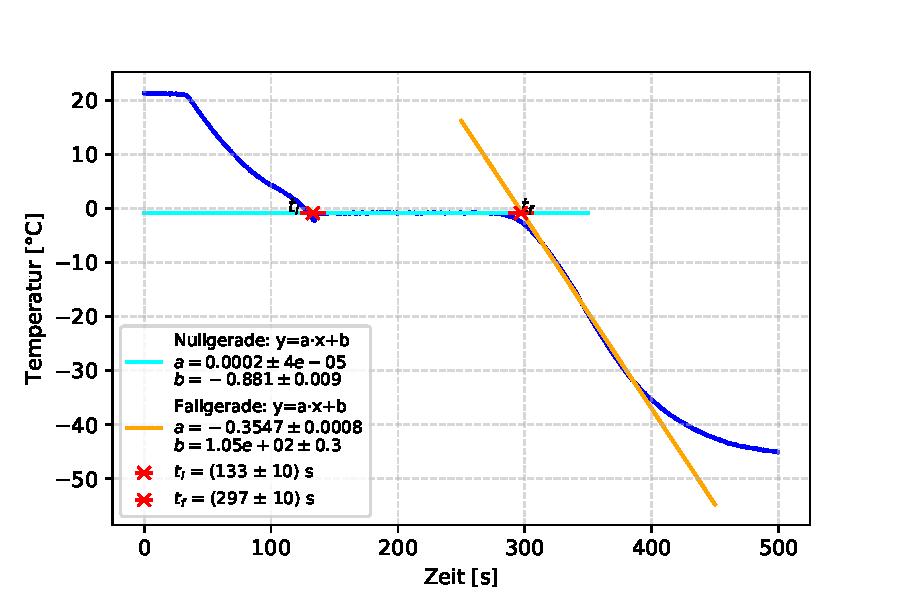
\includegraphics{graphics/plots/Kuelung.pdf}}
    \caption{Plot zur Bestimmung der Start- und Endzeit des Gefriervorgangs}
    \label{fig:GefrierPLT}
\end{figure}

\clearpage
\newpage
\subsection{Der Motor als Wärmekraftmaschine}

\subsubsection{Leerlaufmessung ohne Bremse}

Wir werten nun die Messungen von Versuchsteil Vier aus, wo der Stirlingmotor als Wärmekraftmaschine betrieben wurde. Zunächst werten wir die Leerlaufmessung ohne Bremszaum aus, wobei wir erneut den Wirkungsgrad und eine Energiebilanz betrachten. Danach möchten wir für alle vier vermessenen Bremsstärken den effektiven sowie den thermischen Wirkungsgrad bestimmen und diese Vergleichen. 

Zunächst berechnen wir aber wie bereits einmal gemacht den mittleren Volumenstrom $\dot{V}_2$ aus Tabelle 3 und die Temperaturdifferenz $\Delta T_2$ aus Zu- und Abfluss der Kühlung. Auch berechnen wir den Mittelwert der in Tabelle 4 notierten Flächen der pV-Diagramme $\overline{A}_{pV,leer}$, wobei sich der Fehler analog wie beim Volumenstrom aus dem Standardfehler des Mittelwerts ergibt. Somit erhalten wir:

\begin{equation}
    \begin{split}
        \dot{V}_2 &= (4,819 \pm 0,011) \cdot 10^{-6} \frac{\text{m}^3}{\text{s}}, \\
        \Delta T_2 &= (4,90 \pm 0,14) \text{K}, \\
        \overline{A}_{pV,leer} &= (2,383 \pm 0,017) \text{Pa m}^3.
    \end{split}
\end{equation}

Nun können wir die elektrische sowie abgeführte Leistung $P_{el}$ \& $P_{ab}$ und Wärme $Q_{el}$ \& $Q_{ab}$ bestimmen. Dazu verwenden wir die Gleichungen \ref{eq:Wärmekraftmaschine-Q_el} und \ref{eq:Wärmekraftmaschine-Q_ab}, wobei diese analog zum Fall der Kältemaschine berechnet werden und somit die Fehler auch die gleiche Form annehmen wie in den Rechnungen \ref{eq:3.1-Q_2} und \ref{eq:3.1-Q_1}. Wir erhalten somit:

\begin{equation}
    \begin{split}
        \bm{P_{el}} &= \bm{(167,4 \pm 0,6)} \textbf{W} \\
        \bm{Q_{el}} &= \bm{(33,76 \pm 0,14)} \textbf{J} \\
        \bm{P_{ab}} &= \bm{(98,7 \pm 2,9)} \textbf{W} \\
        \bm{Q_{ab}} &= \bm{(19,9 \pm 0,6)} \textbf{J} \\
    \end{split}
\end{equation}

Nun müssen wir noch die Leistung $P_{pV}$ und Wärme $Q_{pV}$ des Motors bestimmen. Dazu verwenden wir die Fläche des pV-Diagramms $\overline{A}_{pV,leer}$. Die Wärme entspricht einfach genau diesem Wert

\begin{equation}
    \bm{Q_{pV}} = \bm{\overline{A}_{pV,leer}} = \bm{(2,383 \pm 0,017)} \textbf{J},
\end{equation}

während sich die Leistung nun durch Multiplikation mit der gemessenen Motordrehzahl $f_{leer} = (297,5 \pm 0,5)$ 1/min ergibt:

\begin{equation}
    \begin{split}
        P_{pV} &= f_{leer} \cdot \overline{A}_{pV,leer} \\
        \Rightarrow \Delta P_{pV} &= \sqrt{(f_{leer} \cdot \Delta \overline{A}_{pV,leer})^2 + (\overline{A}_{pV,leer} \cdot \Delta f_{leer})^2} \\ \\
        &\Rightarrow \bm{P_{pV} = (2,383 \pm 0,017)} \textbf{W}
    \end{split}
\end{equation}

Somit können wir den thermischen Wirkungsgrad der Leerlaufmessung $\eta_{th,leer}$ aus dem Verhältnis der Motorwärme zur elektrischen Wärme berechnen:

\begin{equation}
    \begin{split}
        \eta_{th,leer} &= \frac{Q_{pV}}{Q_{el}} \\
        \Rightarrow \Delta \eta_{th,leer} &= \eta_{th,leer} \sqrt{\left( \frac{\Delta Q_{pV}}{Q_{pV}} \right)^2 + \left( \frac{\Delta Q_{el}}{Q_{el}} \right)^2} \\ \\
        &\Rightarrow \bm{\eta_{th,leer} = (7,06 \pm 0,06)} \%
    \end{split}
\end{equation}

Ebenso können wir nun nach Gleichung \ref{eq:Wärmekraftmaschine-Verlust} den gesamten Verlust $Q_V$ bestimmen:

\begin{equation}
    \begin{split}
        Q_V &= Q_{el} - Q_{ab} - Q_{pV} \\
        \Rightarrow \Delta Q_V &= \sqrt{(\Delta Q_{el})^2 + (\Delta Q_{ab})^2 + (\Delta Q_{pV})^2} \\ \\
        &\Rightarrow \bm{Q_V = (11,5 \pm 0,6)} \textbf{J}
    \end{split}
\end{equation}

Diese Verluste werden hauptsächlich wieder die Ursache der mangelnden Wärmeisolierung des Motors aufgrund seiner Glaskonstruktion sein. Andererseits werden aber auch Reibungsverluste beim Betrieb des Motors eine Rolle spielen.  

\newpage
\subsubsection{Motor mit Bremszaum}

Wir werten nun die Messungen bei verschiedenen Bremsstärken aus. Dazu gehen wir wie folgt vor:

Zunächst berechnen wir aus den in Tabelle 5 notierten Flächeninhalten $A$ den Durchschnitt $\overline{A}$ für jede Kraft analog zum Leerlauf. Anschließend berechnen wir auch den Mittelwert der jeweils drei Drehzahlmessungen, dessen Fehler sich aus dem Standardfehler des Mittelwerts $\sigma_{std}$ sowie dem notierten Messfehler $\Delta f$ ergibt als $\Delta \overline{f} = \sqrt{\sigma_{std}^2 + \Delta f^2}$. Die Ergebnisse tragen wir in Tabelle \ref{tab:Bremsmessung-Mittel} ein. 


\phantom{.}

\begin{table}[!h]
    \centering
    \resizebox{\textwidth}{!}{
    \begin{tabular}{ccccc}
        \hline
        $\bm{F}$ [N] & $\bm{U_H}$ [V] & $\bm{I_H}$ [A] & $\bm{\overline{A}}$ [Pa m$^3$] & $\bm{\overline{f}}$ [1/s]  \\ \hline
         0,82 $\pm$ 0,03 & 12,3  $\pm$ 0,02 & 13,6 $\pm$ 0,01 & 3,206 $\pm$ 0,006 & 3,727 $\pm$ 0,009 \\
         0,61 $\pm$ 0,03 & 12,32 $\pm$ 0,02 & 13,6 $\pm$ 0,01 & 3,040 $\pm$ 0,012  & 4,186 $\pm$ 0,009 \\
         0,4  $\pm$ 0,03 & 12,31 $\pm$ 0,02 & 13,6 $\pm$ 0,01 & 2,807 $\pm$ 0,014  & 4,728 $\pm$ 0,010 \\
         0,19 $\pm$ 0,03 & 12,3  $\pm$ 0,02 & 13,6 $\pm$ 0,01 & 2,563 $\pm$ 0,022  & 5,086 $\pm$ 0,012  \\ \hline
    \end{tabular}}
    \caption{Messergebnisse der Bremsmessung - gemittelt}
    \label{tab:Bremsmessung-Mittel}
\end{table}

\phantom{.}

Nun berechnen wir für jede der vier Bremsmessungen die elektrische Wärme $Q_{el}$ sowie die mechanischen Arbeitswerte $W_{pV}$ sowie $W_D$. Wir verwenden für erstes die bekannte Formel $Q = UI/f$ und $W_{pV}$ entspricht einfach dem gemittelten Flächeninhalt des pV-Diagramms. Für $W_D$ verwenden wir Gleichung \ref{eq:Wärmekraftmaschine-W_D&P_D}, wobei wir für $l$ die im Skrtipt gegebene Länge von $l= 25$cm einsetzen. Der Fehler berechnet sich somit zu:

\begin{equation}
    \Delta W_D = 2 \pi l \cdot \Delta F.
\end{equation}

Aus diesen Werten kann nun noch jeweils der thermische $\eta_{th}$ und der effektive $\eta_{eff}$ Wirkungsgrad bestimmt werden. Dazu verwenden wir:


\begin{equation}
    \begin{split}
        \eta_{th} &= \frac{W_{pV}}{Q_{el}} \\
        \Rightarrow \Delta \eta_{th} &= \eta_{th} \sqrt{\left( \frac{\Delta W_{pV}}{W_{pV}} \right)^2 + \left( \frac{\Delta Q_{el}}{Q_{el}} \right)^2}
    \end{split}
\end{equation}


\begin{equation}
    \begin{split}
        \eta_{eff} &= \frac{W_D}{Q_{el}} \\
        \Rightarrow \Delta \eta_{eff} &= \eta_{eff} \sqrt{\left( \frac{\Delta W_{D}}{W_{D}} \right)^2 + \left( \frac{\Delta Q_{el}}{Q_{el}} \right)^2}
    \end{split}
\end{equation}

Somit haben wir alles beisammen, was wir benötigen. Die berechneten Ergebnisse sind in Tabelle \ref{tab:Bremsmessung-Wirkungsgrade} zu sehen. 

\phantom{.}

\begin{table}[!h]
    \centering
    \resizebox{\textwidth}{!}{
    \begin{tabular}{cccccc}
        \hline
        \textbf{Nr.} & $\bm{Q_{el}}$ [J] & $\bm{W_{pV}}$ [J] & $\bm{W_D}$ [J] & $\eta_{th}$ [\%] & $\eta_{eff}$ [\%]  \\ \hline
             1 &  44,89 $\pm$    0,13 &  3,206 $\pm$   0,006 & 1,29 $\pm$  0,05 &    7,142 $\pm$   0,025 &      2,87 $\pm$       0,11 \\
             2 &  40,03 $\pm$    0,11 &  3,040  $\pm$   0,012 & 0,96 $\pm$  0,05 &    7,60 $\pm$     0,04 &      2,39  $\pm$       0,12 \\
             3 &  35,41 $\pm$    0,1  &  2,807 $\pm$   0,014 & 0,63 $\pm$  0,05 &    7,93 $\pm$     0,05 &      1,77 $\pm$       0,13 \\
             4 &  32,89 $\pm$    0,1  &  2,563 $\pm$   0,022 & 0,30 $\pm$  0,05 &    7,79 $\pm$     0,07 &      0,91 $\pm$       0,14 \\ \hline
    \end{tabular}}
    \caption{Berechnung der Wirkungsgrade $\eta_{th}$ \& $\eta_{eff}$}
    \label{tab:Bremsmessung-Wirkungsgrade}
\end{table}

\phantom{.}

Zum Vergleich werden $\eta_{th}$ und $\eta_{eff}$ als Funktionen der Frequenz in eine Diagramm aufgetragen, Abbildung \ref{fig:WirkungsgradePLT}, um den Verlauf zu interpretieren. Hier wird auch nochmal gut die deutliche Differenz zwischen den beiden Wirkungsgraden klar. Diese erklärt sich folgendermaßen:

$W_{pV}$ bezeichnet die pure im Kreisprozess erzeugte Arbeit, basierend auf den Druck- und Volumemessungen im Zylinder, während $W_D$ den Anteil der gesamten zugeführten Arbeit von der Heizwendel bezeichnet, die dem Motor durch die Bremsung verloren geht. Somit steht $\eta_{th}$ für den theoretischen Wirkungsgrad basierend auf der grundsätzlichen Leistung der Maschine und $\eta_{eff}$ für den Wirkungsgrad der Gegenwirkung zur Bremsung. Somit erklärt sich auch, weshalb der effektive Wirkungsgrad deutlich kleiner ist. Wären die Wirkungsgrade nämlich gleich groß, so würde das einen Stillstand des Motors erzeugen. Eine Bewegung setzt also voraus, dass der effektive kleiner als der thermische ist.

Eine weitere interessante Beobachtung ist, dass der thermische Wirkungsgrad bei zunehmender Drehfrequenz zu steigen und zugleich der effektive Wirkungsgrad abzufallen scheint. Hauptgrund ist hierbei, dass die Reibungsverluste mit zunehmender Drehzahl abnehmen und somit der Wert von $W_D$ geringer wird. Im Gegenzug ist im thermischen Wirkungsgrad der erwartete Verlauf zu erkennen, dass bei größerer Drehzahl die Leistung und somit der Wirkungsgrad steigt. So entstehen die entgegengesetzten Verläufe bei steigender Drehfrequenz.  

\begin{figure}[!p]
    \centering
    \resizebox{\textwidth}{!}{
    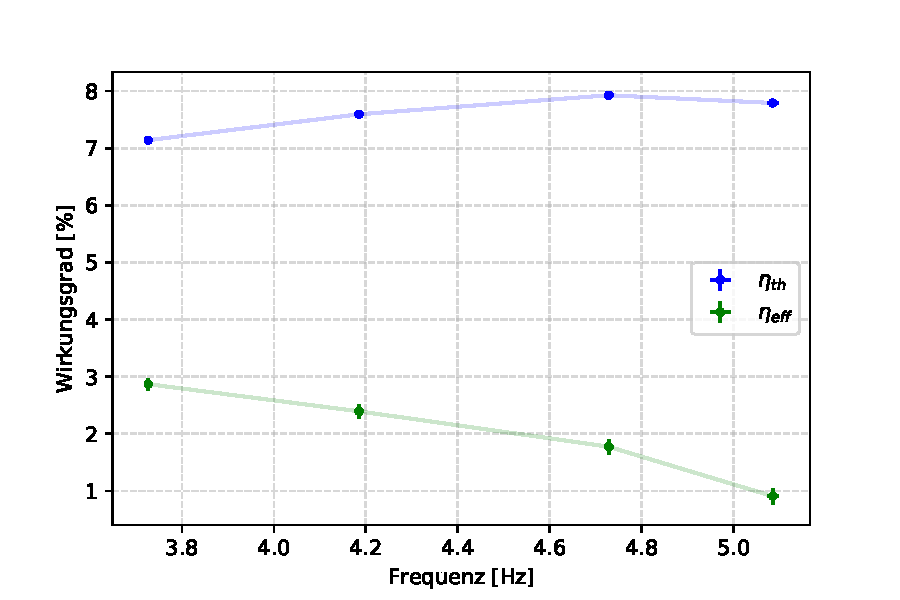
\includegraphics{graphics/plots/Wirkungsgrade-1.pdf}}
    \caption{Thermischer und Effektiver Wirkungsgrad bei unterschiedlichen Frequenzen}
    \label{fig:WirkungsgradePLT}
\end{figure}

\clearpage
\newpage
%---------------PRÄSENTATION DER ENDERGEBNISSE---------------
\section{Zusammenfassung der Endergebnisse}

Wir begannen, indem wir mithilfe Kompensationsmessung  die Kühlleistung des als Kältemaschine laufenden Stirling-Motors bestimmten, den Wirkungsgrad bestimmten und eine Energiebilanz austellten. Die Leistung und der Wirkungsgrad ergaben sich dabei zu:

\begin{equation}
    \begin{split}
        \bm{P_1} &= \bm{(30,23 \pm 0,27)} \textbf{W}, \\
        \bm{\eta_1} &= \bm{(74,1 \pm 2,3)} \%.
    \end{split}
\end{equation}

Die Energiebilanz zeigte eine signifikante Abweichung von $\sigma_{zu, ab} = 4,08$ zwischen der abgebebenen Wärme zu der geleisteten Arbeit mit reingesteckter Wärme. Diese Verluste ließen sich auf die Reibung und ungewollten Wärmeaustausch zurückführen und wirken von der Größenordnung her sinnvoll im Kontext des berechneten Wirkungsgrads.

Daraufhin analysierten wir den Temperaturverlauf von Wasser in einem in den Motor eingebrachten Reagenzglas einmal beim Abkühlen auf bis zu ca. -45°C und beim darauf folgenden Erwärmen auf ungefähr 100°C. Hier konnten deutlich die Übergangszeiten zwischen den Aggregatzuständen bei 0°C beobachtet werden, welche beim Erwärmen deutlich kürzer waren als beim Abkühlen aufgrund des Wärmeaustauschs mit der höheren Raumtemperatur. Aus der abgelesenen Gefrierzeit bestimmten wir erneut die Kühlleistung des Motors:

\begin{equation}
    \bm{P_2} = \bm{(2,04 \pm 0,20)} \textbf{W}.
\end{equation}

Dieser Wert weicht sehr signifikant vom zuvor berechneten Wert $P_1$ ab mit einer Abweichung von $\sigma_P = 82,68$, welche mit der bereits diskutierten Arbeit gegen die Raumtemperatur begründet werden kann.

Im Letzten Versuchsteil nutzten wir den Motor als Wärmekraftmaschine, wobei wir zunächst eine Leerlaufmessung beobachteten. Hauptergebnisse der Auswertung waren hier der thermische Wirkungsgrad im Leerlauf sowie eine Berechnung der gesamten Wärmeverluste:

\begin{equation}
    \begin{split}
        \bm{\eta_{th,leer}} &= \bm{(7,06 \pm 0,06)} \% \\
        \bm{Q_V} &= \bm{(11,5 \pm 0,6)} \textbf{J}
    \end{split}
\end{equation}

Die Verluste wurden hier erneut auf den Wärme- und Reibungsverlust zurückgeführt. 

Anschließend beobachteten wir die Wärmekraftmaschine bei vier unterschiedlich starken angelegten Bremsstärken und bestimmten für jeden der vier Fälle den thermischen und effektiven Wirkungsgrad:

\begin{table}[!h]
    \centering
    \begin{tabular}{ccc}
        \hline
        \textbf{Nr.} & $\eta_{th}$ [\%] & $\eta_{eff}$ [\%]  \\ \hline
             1 &    7,142 $\pm$     0,025 &      2,87 $\pm$       0,11 \\
             2 &    7,60 $\pm$     0,04 &      2,39  $\pm$       0,12 \\
             3 &    7,93 $\pm$     0,05 &      1,77 $\pm$       0,13 \\
             4 &    7,79 $\pm$     0,07 &      0,91 $\pm$       0,14 \\ \hline
    \end{tabular}
    \caption{Zusammenfassung Wirkungsgrade $\eta_{th}$ \& $\eta_{eff}$}
\end{table}

Zum Vergleich wurden diese Werte in ein Diagramm in Abhängigkeit der jeweils gemessenen Drehfrequenz des Motors aufgetragen. Hier konnte beobachtet werden, dass der effektive Wirkungsgrad der Bremsung deutlich kleiner ist als der thermische und mit steigender Frequenz aufgrund der abnehmenden Reibungsverluste abfällt.

\newpage
%---------------ZUSAMMENFASSUNG UND DISKUSSION---------------
\section{Diskussion}

Allgemein wurden beim Versuch durchaus erwartete und sinnvolle Ergebnisse erzielt. Das die Ergebnisse der Wirkungsgrade zwar generell sehr klein und somit die Abweichungen der Energibilanzen sehr hoch sind ist zwar zunächst etwas erschreckend, im Kontext des Versuchsaufbaus und dem verwendeten Motor aber durchaus realistisch. Der größte Punkt wird wie bereits mehrfach erwähnt die Glaskonstruktion des Motors sein, welche einen sehr hohen Verlust aufgrund von Wärmeabstrahung und -leitung aufweist. Jedoch diente die Glaskonstruktion vor allem dem Demonstrationszweck im Kontext des Physikalischen Anfängerpraktikums, weshalb eine isolierendere Konstruktion zwar effizienter, aber dafür bei weitem nicht so spektakulär und interessant zu beobachten wäre. Somit ist der Glasaufbau im Gesamtkontext deutlich besser für diesen Versuch geeignet, auch wenn dafür die Ergebnisse deutlich weiter auseinanderliegen und die Leistung erheblich gesenkt wird. Als weiterer Ausgleich konnte zudem eine ausführlichere Auseinandersetzung und Interpretation der Ergebnisse bei der Ursachenfindung für Verluste erfolgen. 

Ein Aspekt, der die Ergebnisse trotz der Glaskonstruktion aber nochmal deutlich verbessert haben wird, ist die Verwendung des eingebauten Regenerators. Es wurde zwar keinerlei Vergleichsmessung mit einem Motor ohne Regenerator zur genaueren quantitativen Analyse des Effekts vorgenommen, jedoch lässt sich aus den Grundlagen herleiten, dass dieser einen deutlich Einfluss auf die Effektivität des Motors gehabt haben wird. 

Des Weiteren wird die großzügige und großflächige Unterstützung der Messung von technischen Geräten einen positiven Effekt auf die Ergebnisse haben. Da praktisch in keiner Form manuell irgendein Wert gemessen werden musste, sondern alle einfach nur von den digitalen Geräten abgelesen werden mussten, werden statistische Messfehler basierend auf menschlichen Fehlern effektiv minimiert. Doch auch abgesehen davon lässt sich feststellen, dass alle manuell einzustellenden Sachen während des Versuchs, wie beispielsweise die Regulierung der Heizung auf Raumtemperatur im ersten Teil, vergleichsweise gut geklappt haben und somit keine größeren Fehler hiervon zu erwarten wären. 

Es wird also nochmal deutlich, dass die großen Abweichungen in der Auswertung mit geringen Wirkungsgraden und fast schon katastrophalen Energiebilanzen nicht das Resultat irgendeines gravierenden Messfehlers sind, sondern vielmehr aufzeigen, wie weit die Realität hier doch vom theoretisch idealen Fall entfernt ist, wie groß die Verluste in einem Motor sind und wie wichtig eine gute thermische Isolierung wird, wenn man wirklich effektiv Leistung mit einem Motor erzeugen möchte.

Zusammenfassend lässt sich also sagen, dass der Versuch flächendeckend realistische Ergebnisse erzielte, die einen aussagekräftigen Kontrast zur Theorie darstellen. Somit war der Versuch eine interessante und lehrreiche Einführung in die Welt der Motoren und Maschinen, die die Komplexität des Themas aufzeigt und die Schwierigkeiten bei der Suche nach dem perfekten Motor klar macht.



\newpage
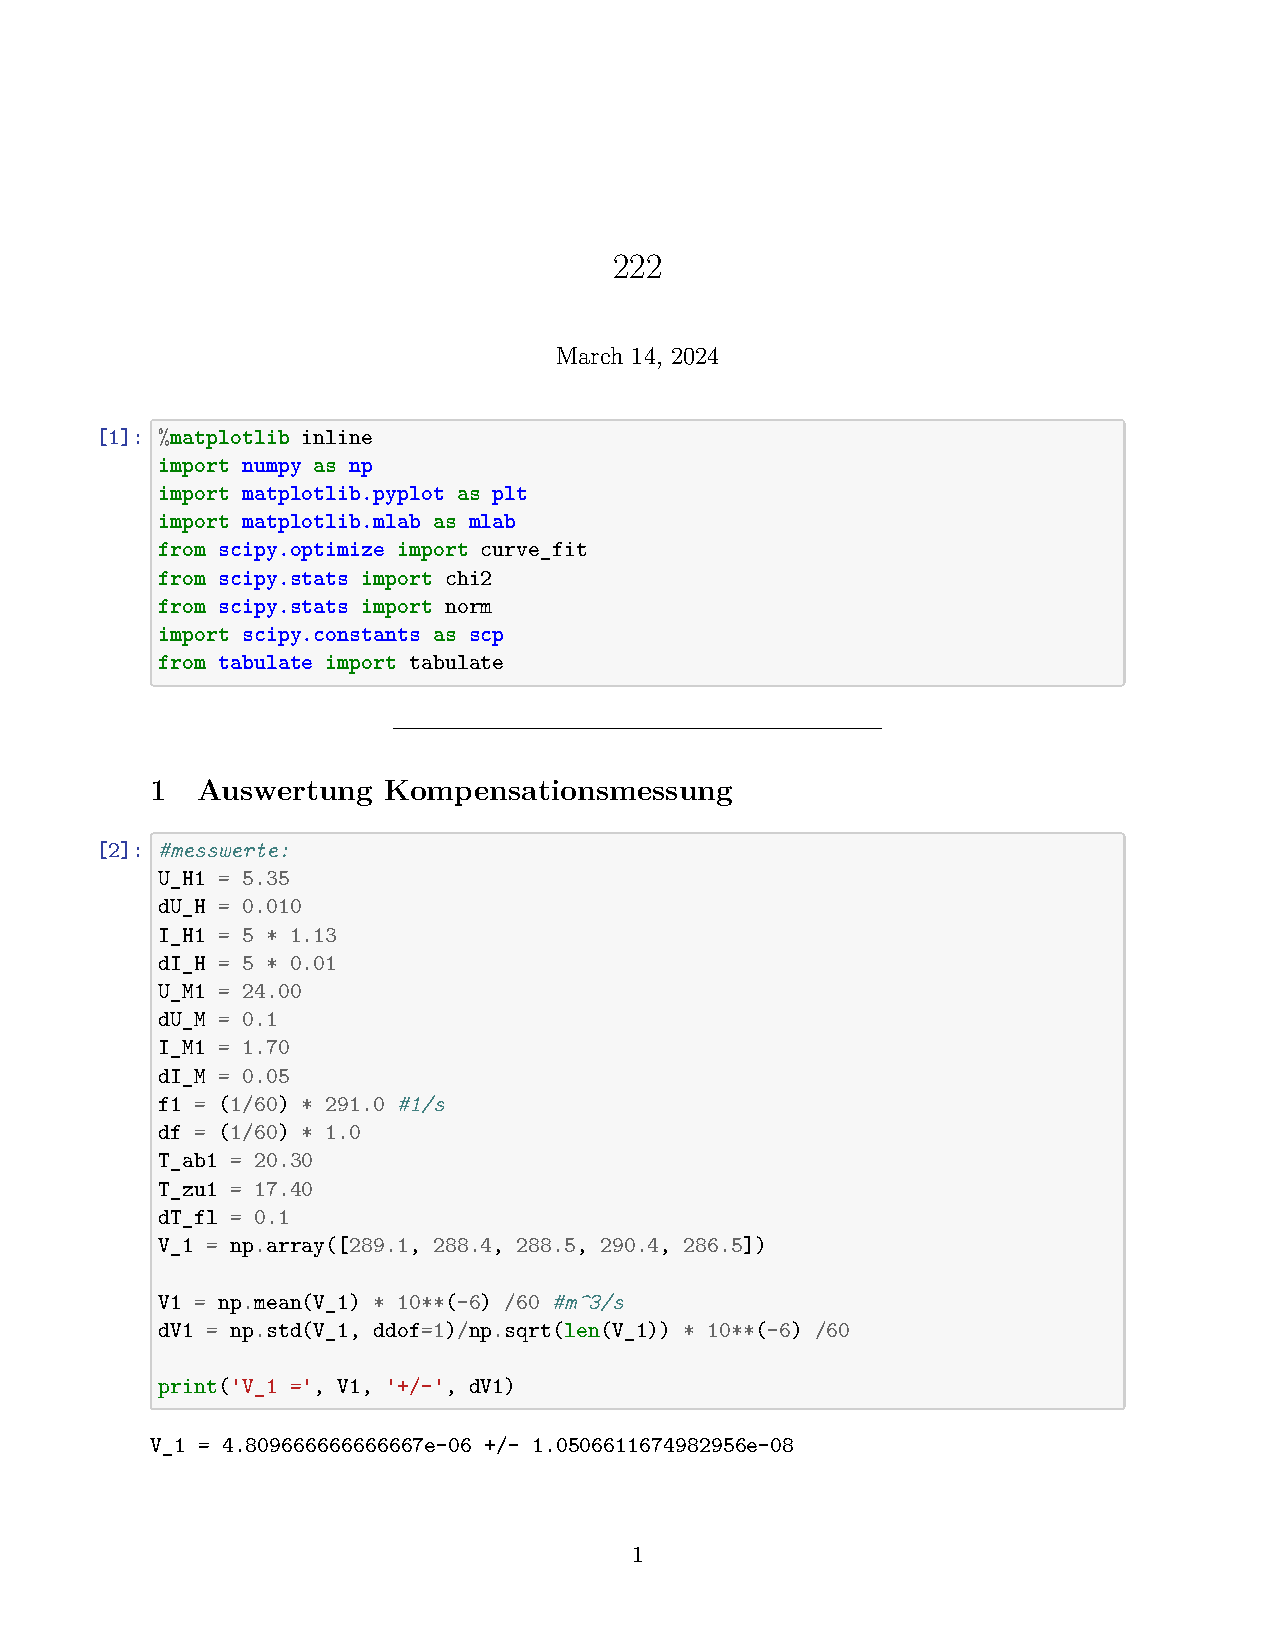
\includepdf[pages=-]{222-1.pdf}

\end{document}

